\documentclass{article}

\renewcommand{\abstractname}{Individual Assignment 2}

% Set page size and margins
% Replace `letterpaper' with`a4paper' for UK/EU standard size
\usepackage[a4paper,top=1.5cm,bottom=1.5cm,left=2cm,right=2cm,marginparwidth=1cm]{geometry}

% Useful packages
\usepackage{amsmath}
\usepackage{graphicx}
\usepackage[colorlinks=true, allcolors=blue]{hyperref}
\usepackage[tbtags]{amsmath} % for math
\usepackage{minted}
\usepackage{indentfirst}

\title{BAM - AS\&P}
\author{Aleksander Odziemkowski}

\begin{document}
\maketitle

\begin{abstract}
\centering
\end{abstract}

\section{Difference-in-difference (DiD) analysis}

\subsection{Delineation of the problem and dataset}

The first chapter focuses on estimating the effects of the 1993 policy intervention in the form of Earned Income Tax Credit (EITC) on labor supply for single women by condition on whether or not they had children. The EITC is a refundable
tax credit for low-income workers installed in the US which aimed at stimulating female labor participation.

The dataset used in this part of the document consists of 13,746 observations across 11 variables. Data points pertain to single women in US in the age of 20-54 with less than high-school education covering the years 1991 to 1996.

The year of intervention in question is 1993. For the sake of difference-in-difference (DiD) analysis, observations for years 1991 and 1992 are considered to reflect the period prior to intervention whilst observations from 1993 and beyond serve to reflect the post-intervention state of the matter. Moreover, it is assumed that all women observed in the data set remain in the same state across the variables for the period in question. 

The EITC intervention effect will be measured by the change of mean value of three variables for treatment and control groups: indicator of work status (\emph{work}), annual earnings (\emph{earn}) and family income (\emph{finc}). Treatment and control group are assigned based on a subject having children (treatment) and not having them (control).

\subsection{Canonical difference-in-difference equation}
\label{canonical}

The following is considered to be a canonical difference-in-difference equation:

\begin{equation}
    y_{it}\ =\ \beta_0\ +\ \beta_1D_i\ +\ \beta_2T_t\ +\ \beta_3{D_iT}_t\ +\ \varepsilon_{it}
\end{equation}

Below are the expectation operators E(.) from probability space which indicate possible outcomes in the DiD analysis and are assigned to coefficients from the canonical DiD equation above:

\begin{itemize}
    \item $E\ =\ (y_{T\ =\ 1}\ |\ D\ =\ 1)$ corresponds with $y_{it}\ =\ \beta_0\ +\ \beta_1+\ \beta_2+\ \beta_3$
    \item $E\ =\ (y_{T\ =\ 0}\ |\ D\ =\ 1)$ corresponds with $y_{it}\ =\ \beta_0\ +\ \beta_1$
    \item $E\ =\ (y_{T\ =\ 1}\ |\ D\ =\ 0)$ corresponds with $y_{it}\ =\ \beta_0\ +\beta_2$
    \item $E\ =\ (y_{T\ =\ 0}\ |\ D\ =\ 0)$ corresponds with $y_{it}\ =\ \beta_0$
\end{itemize}

The substitution of terms yields the following simplification/condensation of the difference-in-difference effect:

\begin{equation}
    [E(y_{T\ =\ 1}\ |\ D\ =\ 1) - E(y_{T\ =\ 0}\ |\ D\ =\ 1)] - [E(y_{T\ =\ 1}\ |\ D\ =\ 0) - E(y_{T\ =\ 0}\ |\ D\ =\ 0)]
\end{equation}

\begin{equation}
    {[(\beta}_0\ +\ \beta_1+\ \beta_2+\ \beta_3)\ -\ (\beta_0\ +\ \beta_1)] - [(\beta_0\ + \beta_2)\ - (\beta_0)]\ = (\beta_2+\ \beta_3)\ - (\beta_2)\ = \beta_3\
\end{equation}

\subsection{Graphical evidence of DiD effect of the EITC introduction}

The DiD effect can also be examined in graphical representation of the linear development of the dependent variable that measures the effect of EITC across time frame in question. The coefficient singled out in the canonical equation condensation, and so the DiD effect, is nothing else than a change of slope and intercept of the equation in response to the intervention.

\hyperref[fig:earnings]{Figure 1} depicts the response of both treatment and control group to the intervention in 1993 in terms of mean annual earnings per group. It is worth noting that single women without children are on average earning more than those with children (dark blue line placed higher than the light blue line). However, it is evident that after the intervention in 1993 the effect of tax refund in the form of increasing earnings is stronger for women with children. 

\begin{figure}[!htbp]
    \caption{Visual evidence of EITC intervention in terms of annual earnings.}
    \centering
    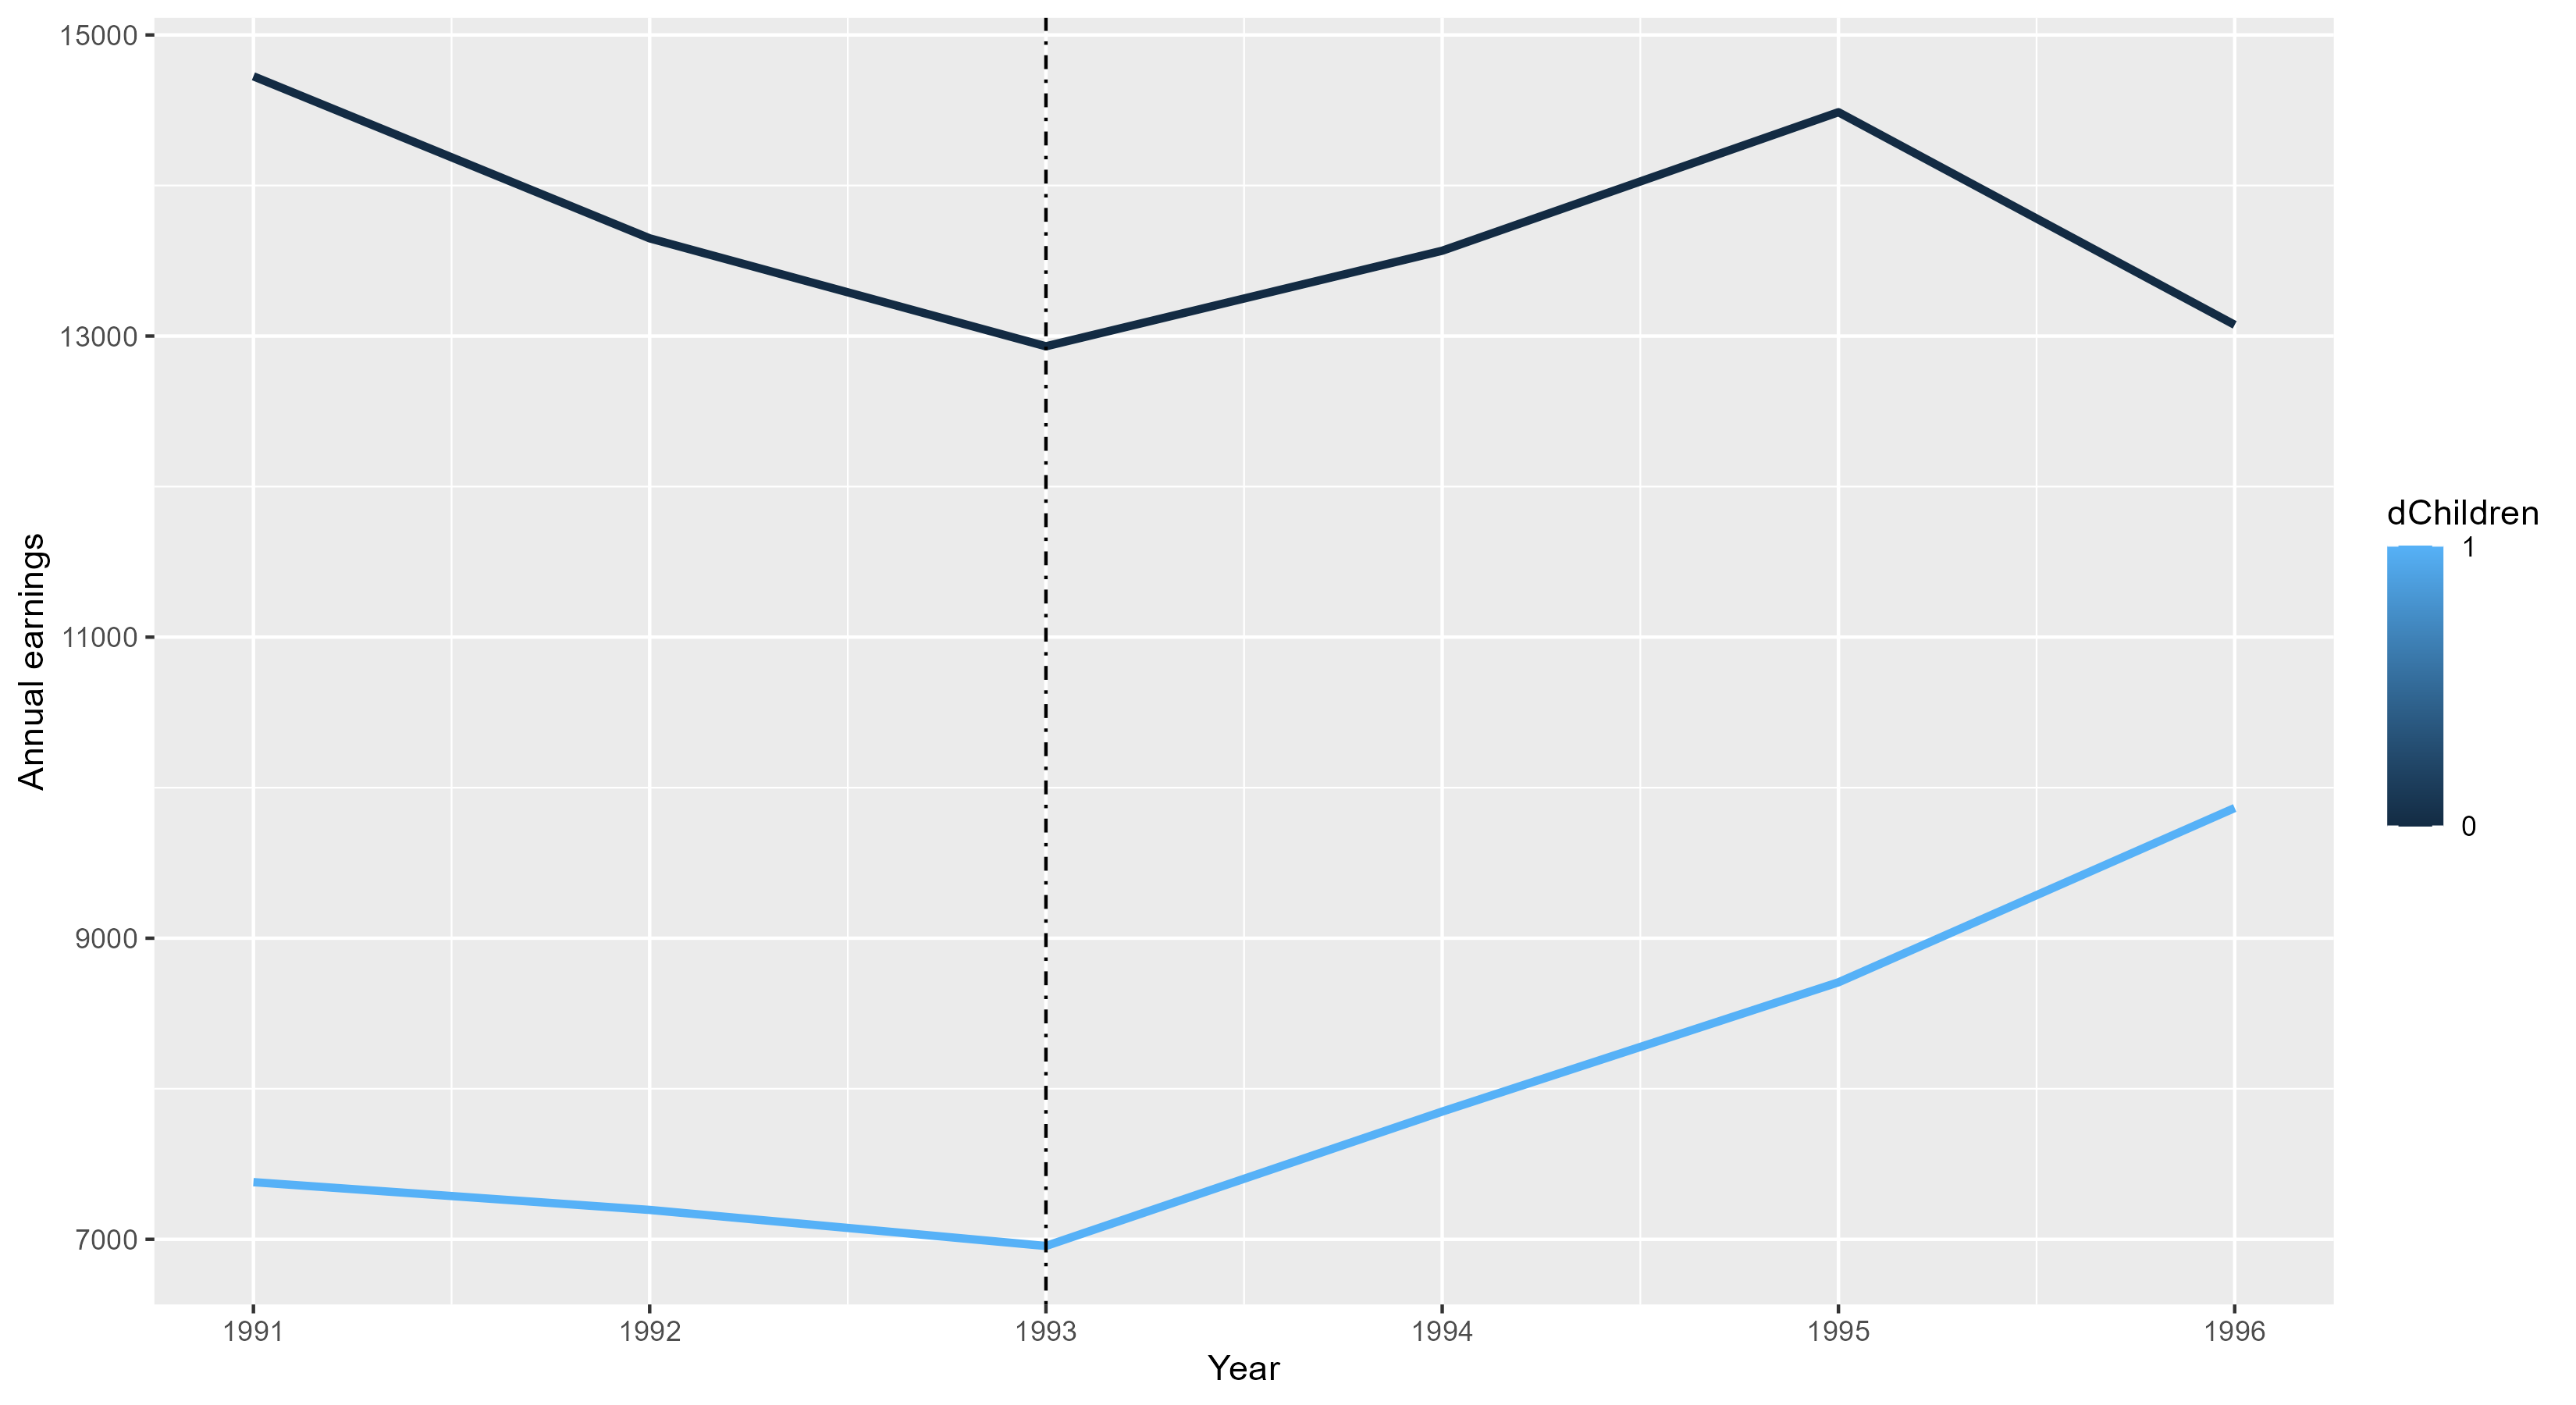
\includegraphics[width=0.6\textwidth]{lineEarnEffect.png}
    \label{fig:earnings}
\end{figure}

In terms of family annual income, the effect of introducing tax refund for single mothers in 1993 is also evidently visible in \hyperref[fig:family]{Figure 2}. The response appears to be less linear, but the same can be inferred from both figures.  

\begin{figure}[!htbp]
    \caption{Visual evidence of EITC intervention in terms of annual earnings.}
    \centering
    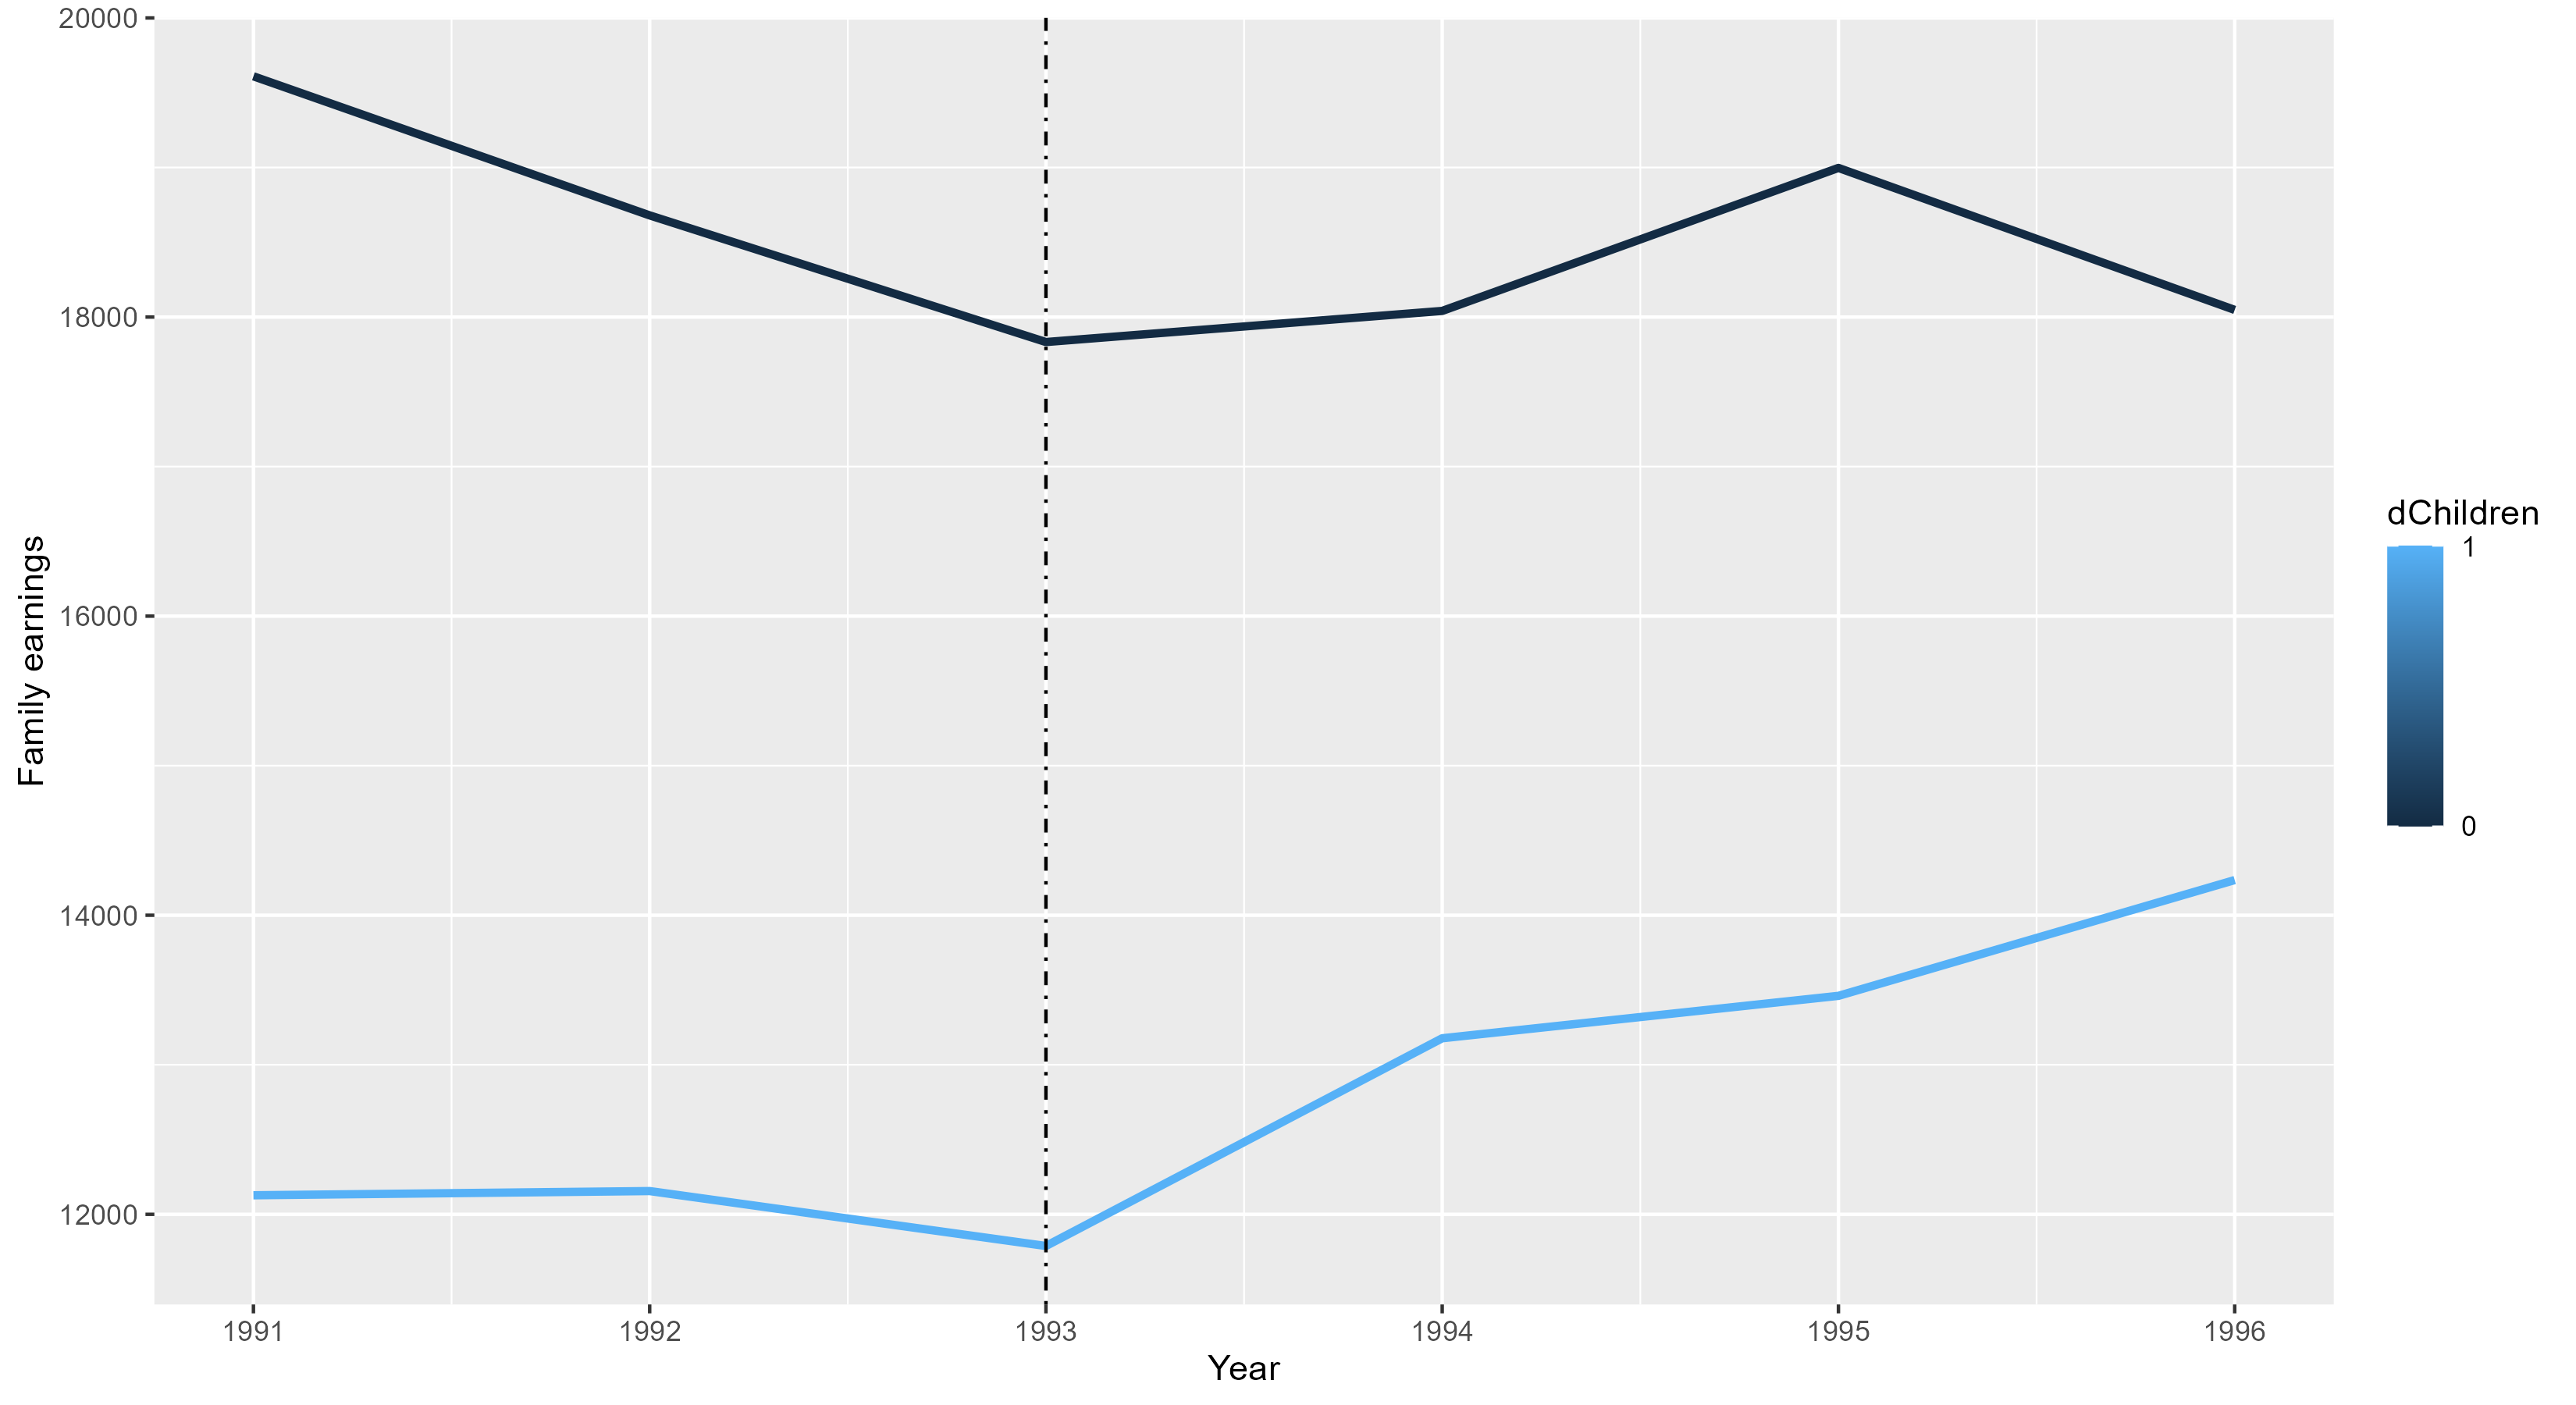
\includegraphics[width=0.6\textwidth]{lineFincEffect.png}
    \label{fig:family}
\end{figure}

It is interesting to look at the EITC introduction effect in terms of employment status of women observed in the dataset. This indicator of work status differs in its nature from two previous variables. Even sharper response to the intervention by the treatment group can be observed in \hyperref[fig:work]{Figure 3}. 

This visual evidence suggests that the difference in response to the tax refund introduced in 1993 in terms of employment status should differ significantly between mothers and childless single women in favor of the former.

\begin{figure}[!htbp]
    \caption{Visual evidence of EITC intervention in terms of annual earnings.}
    \centering
    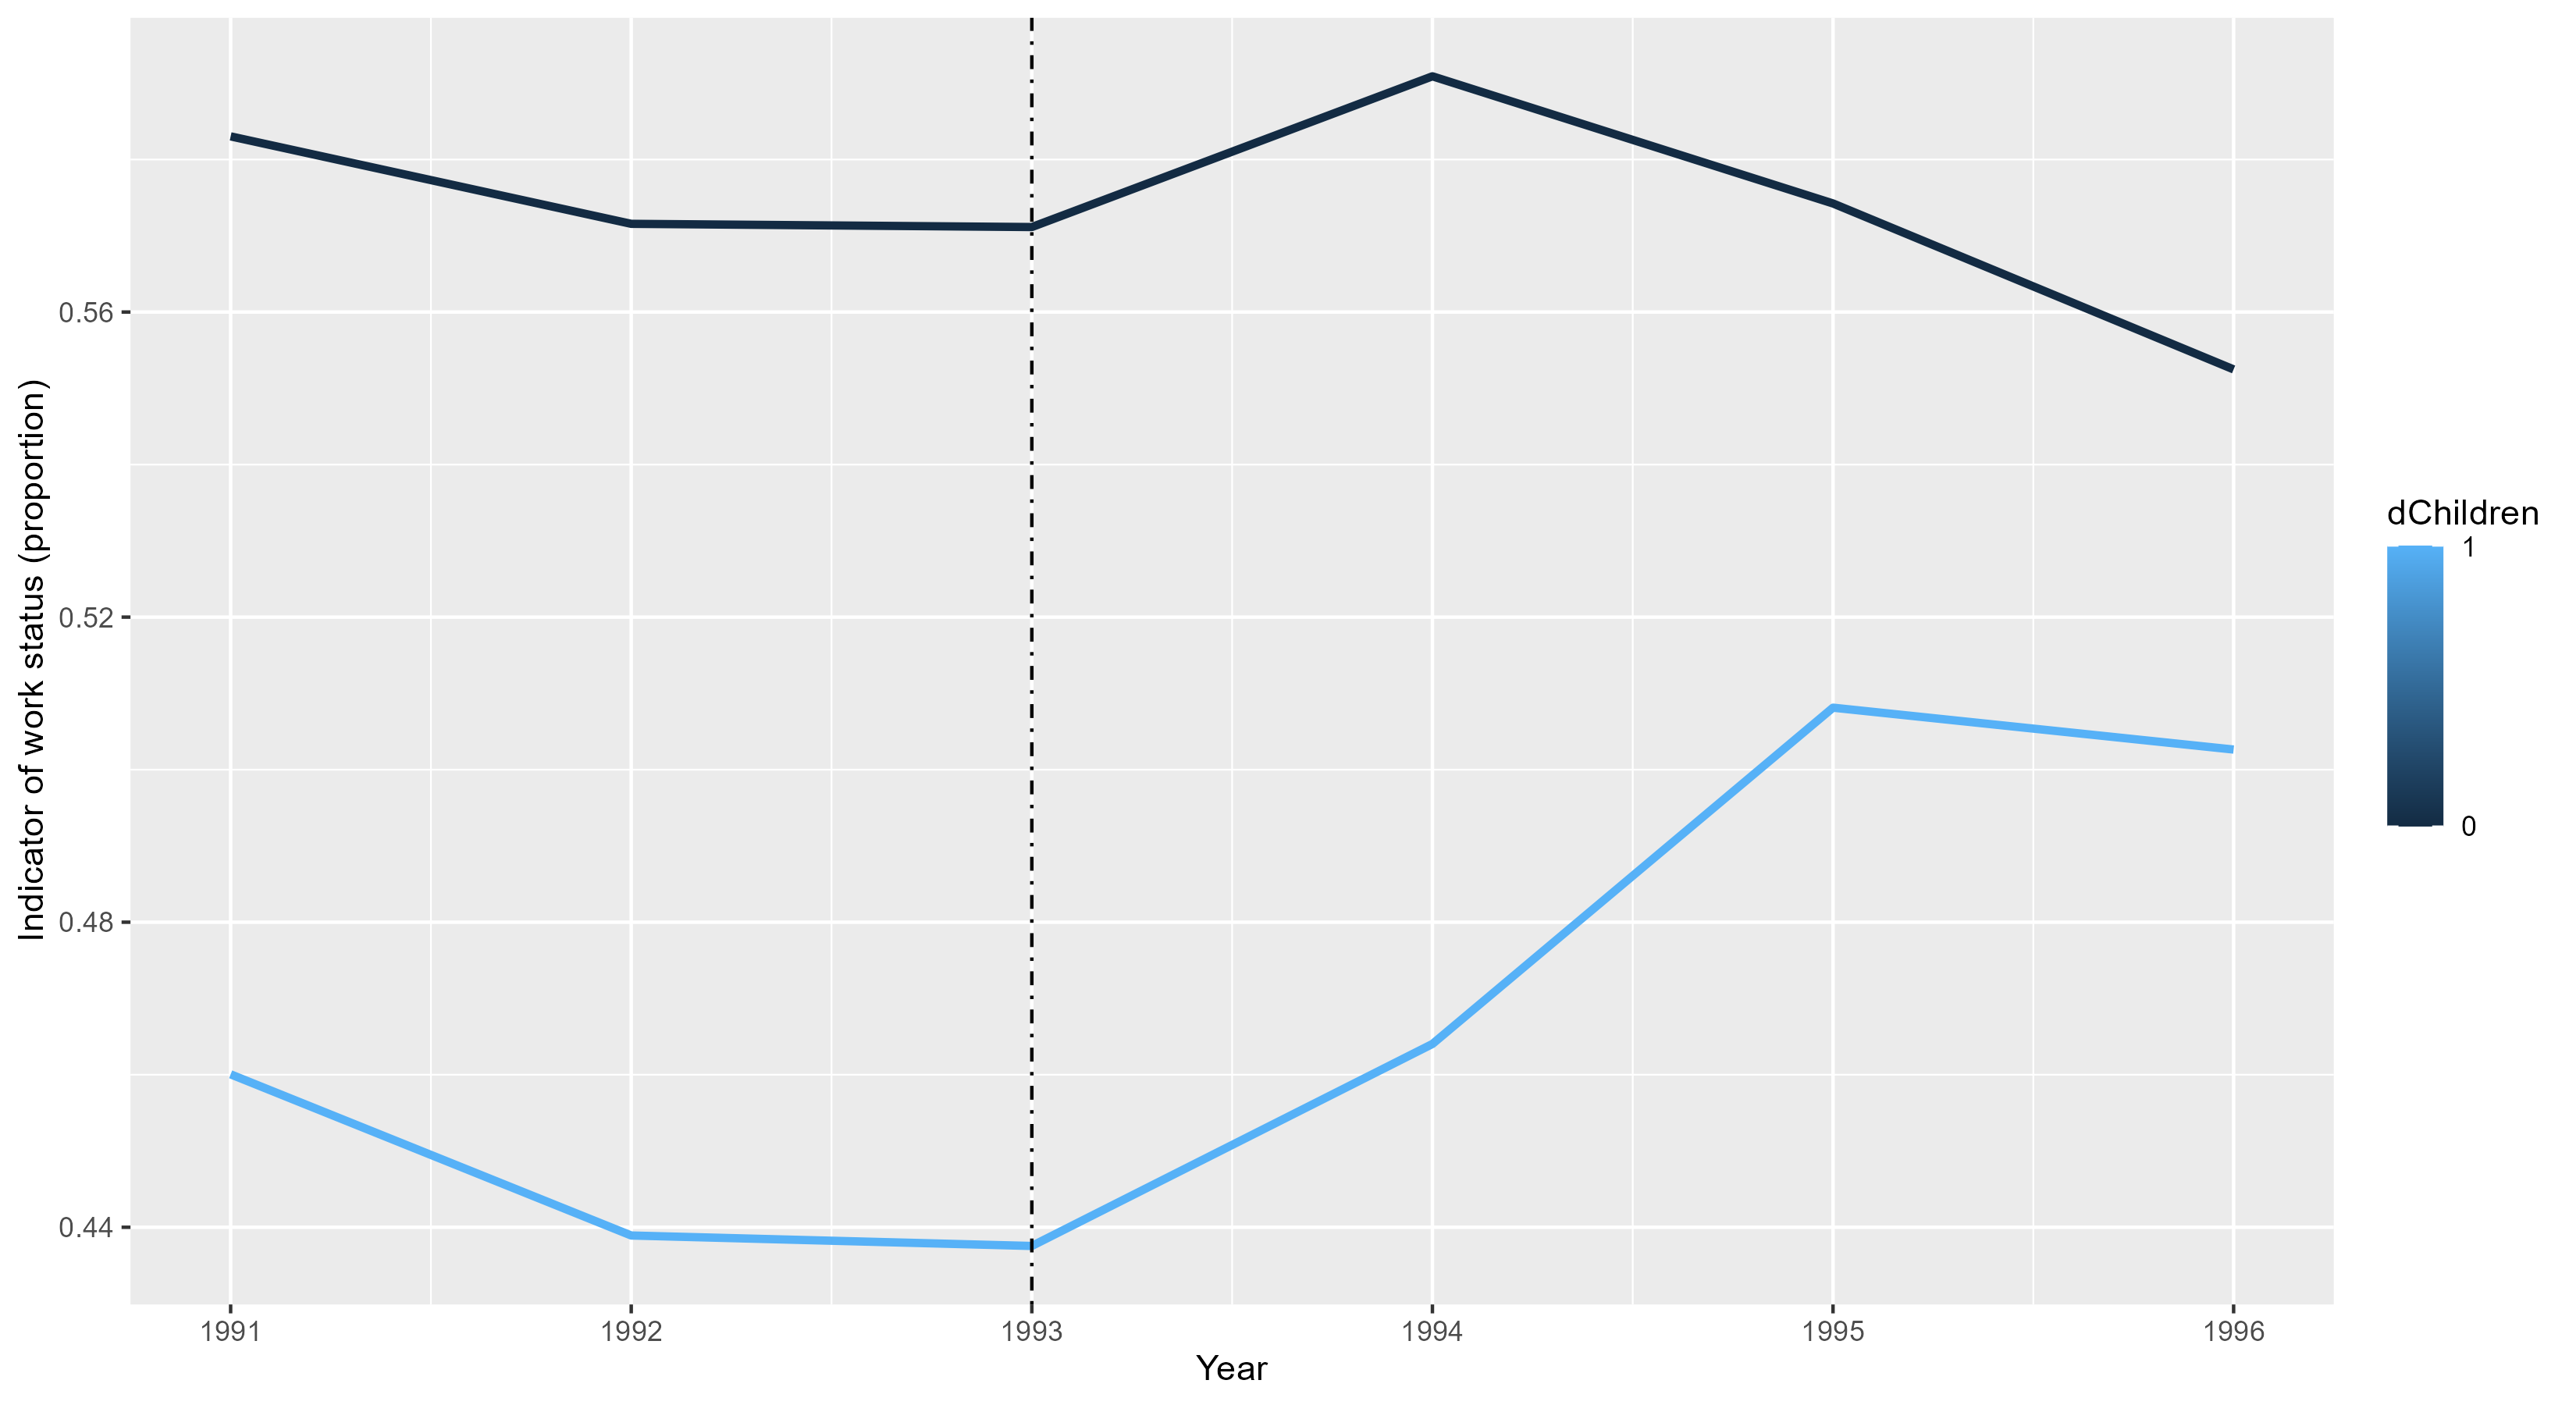
\includegraphics[width=0.6\textwidth]{lineWorkEffect.png}
    \label{fig:work}
\end{figure}


\subsection{Summary statistics}

Below in \hyperref[tab:descriptive]{Table 1} are the summary statistics of the variables used in the subsequent DiD analysis. Worth noting is the skewness of the monetary dependent variables, family income and personal earnings. Such high standard deviation in relation to the mean value is expected with income metrics as very often outliers skew the distribution meaningfully. This can be observed in the range for \emph{earn}[0.00; 537,880.60] and \emph{finc}[0.00; 575,616.80].

Looking at the \emph{dChildren}, it can be observed by the means of mean value that proportion of women with children is higher that those without. Moreover, the work status indicator \emph{work} suggests that the dataset is split in half among working and non-working women.  

Later in the document the unemployment rate per state (\emph{urate}) and race indicator (\emph{nonwhite}) will be used as control variables. The former is characterised by rather small dispersion and little skewness, while the latter suggests that women of non-white race are a majority (60-40) in the dataset.

\begin{table}[!htbp]
\centering
\caption{\label{tab:descriptive} Summary statistics of the variables in dataset.}
\begin{tabular}{@{\extracolsep{5pt}}lccccccc} 
\\[-1.8ex]\hline 
\hline \\[-1.8ex] 
Statistic & \multicolumn{1}{c}{Mean} & \multicolumn{1}{c}{St. Dev.} & \multicolumn{1}{c}{Min} & \multicolumn{1}{c}{Pctl(25)} & \multicolumn{1}{c}{Median} & \multicolumn{1}{c}{Pctl(75)} & \multicolumn{1}{c}{Max} \\ 
\hline \\[-1.8ex] 
urate & 6.76 & 1.46 & 2.60 & 5.70 & 6.80 & 7.70 & 11.40 \\ 
children & 1.19 & 1.38 & 0 & 0 & 1 & 2 & 9 \\ 
nonwhite & 0.60 & 0.49 & 0 & 0 & 1 & 1 & 1 \\ 
finc & 15,255.32 & 19,444.25 & 0.00 & 5,123.42 & 9,636.66 & 18,659.18 & 575,616.80 \\ 
earn & 10,432.48 & 18,200.76 & 0.00 & 0.00 & 3,332.18 & 14,321.22 & 537,880.60 \\ 
age & 35.21 & 10.16 & 20 & 26 & 34 & 44 & 54 \\ 
ed & 8.81 & 2.64 & 0 & 7 & 10 & 11 & 11 \\ 
work & 0.51 & 0.50 & 0 & 0 & 1 & 1 & 1 \\ 
unearn & 4.82 & 7.12 & 0.00 & 0.00 & 2.97 & 6.86 & 134.06 \\ 
dPeriod & 0.63 & 0.48 & 0 & 0 & 1 & 1 & 1 \\ 
dChildren & 0.57 & 0.50 & 0 & 0 & 1 & 1 & 1 \\ 
\hline \\[-1.8ex] 
\end{tabular} 
\end{table} 


\subsection{Evaluation matrices for DiD effects}
\label{matrices}

Following the procedure presented in the lecture, this section evaluates the difference-in-difference effect of EITC introduction with a concise matrix summary where results in terms of average effect value for pre- and post-periods are split among treatment and control groups. 

\begin{table}[!htbp]
\centering
\caption{\label{tab:tmpWork} Matrix summarizing DiD effect in terms of indicator of work status.}
\begin{tabular}{@{\extracolsep{5pt}} D{.}{.}{-3} D{.}{.}{-3} D{.}{.}{-3} D{.}{.}{-3} } 
\\[-1.8ex]\hline 
\hline \\[-1.8ex] 
\multicolumn{1}{c}{} & \multicolumn{1}{c}{dPeriod} & \multicolumn{1}{c}{No children} & \multicolumn{1}{c}{Had children} \\ 
\hline \\[-1.8ex] 
\multicolumn{1}{c}{Pre-effect} & 0 & 0.577 & 0.450 \\ 
\multicolumn{1}{c}{Post-effect} & 1 & 0.573 & 0.476 \\ 
\multicolumn{1}{c}{Difference} &  & -0.005 & 0.026 \\ 
\hline \\[-1.8ex] 
\end{tabular} 
\end{table}

\hyperref[tab:tmpWork]{Table 2} provides information on the difference in average values of the work status (employed vs. unemployed) grouped by single women with and without children with regards to 1993 as a year of tax refund intervention. Basically, after the intervention the average employment rate among women with children has risen by 2.6\% whilst childless single women have on average been employed less by 0.5\%. In principle, the difference-in-difference effect equals 3.1\% (percent reflect the change of proportion between employed (+) and unemployed (-)).

\begin{table}[!htbp]
\centering
\caption{\label{tab:tmpEarn} Matrix summarizing DiD effect in terms of annual earnings.}
\begin{tabular}{@{\extracolsep{5pt}} D{.}{.}{-3} D{.}{.}{-3} D{.}{.}{-3} D{.}{.}{-3} } 
\\[-1.8ex]\hline 
\hline \\[-1.8ex] 
\multicolumn{1}{c}{} & \multicolumn{1}{c}{dPeriod} & \multicolumn{1}{c}{No children} & \multicolumn{1}{c}{Had children} \\ 
\hline \\[-1.8ex] 
\multicolumn{1}{c}{Pre-effect} & 0 & 14,203.900 & 7,290.383 \\ 
\multicolumn{1}{c}{Post-effect} & 1 & 13,507.900 & 8,277.196 \\ 
\multicolumn{1}{c}{Difference} &  & -695.997 & 986.813 \\ 
\hline \\[-1.8ex] 
\end{tabular} 
\end{table} 

Difference-in-difference effect measured by the dependent variable \emph{earn} is equal to the mean change in annual earnings for the single women with children after EITC introduction minus the mean change in annual earnings for the single women without children after said intervention. \hyperref[tab:tmpEarn]{Matrix above} deems the DiD effect to be 1,911.04 in monetary units (970.796 - (-940.239)). All in all, it means that the treatment group has observed positive effects of the tax refund while at the same time the control group has observed the decline in personal annual earnings. This pattern follows the findings outlined in \hyperref[tab:tmpWork]{Table 2}.

\begin{table}[!htbp]
\centering
\caption{\label{tab:tmpEarn} Matrix summarizing DiD effect in terms of family income.}
\begin{tabular}{@{\extracolsep{5pt}} D{.}{.}{-3} D{.}{.}{-3} D{.}{.}{-3} D{.}{.}{-3} } 
\\[-1.8ex]\hline 
\hline \\[-1.8ex] 
\multicolumn{1}{c}{} & \multicolumn{1}{c}{dPeriod} & \multicolumn{1}{c}{No children} & \multicolumn{1}{c}{Had children} \\ 
\hline \\[-1.8ex] 
\multicolumn{1}{c}{Pre-effect} & 0 & 19,159.190 & 12,140.900 \\ 
\multicolumn{1}{c}{Post-effect} & 1 & 18,218.950 & 13,111.690 \\ 
\multicolumn{1}{c}{Difference} &  & -940.239 & 970.796 \\ 
\hline \\[-1.8ex] 
\end{tabular} 
\end{table}

The effect of EITC installment measured by family income tells the same story as with other dependent variables. The results are very close to what can be seen in \hyperref[tab:tmpEarn]{Table 3} for annual earnings, though they are slightly magnified in both directions respectfully. This is due to the fact the if a women has an unearned income or has a partner contributing to the family income, it will always increase her family income in respect to annual earnings, and never decrease it. Overall, difference-in-difference effect is equal to 1,682.81 in monetary units (986.813 - (-695.997)). 986.813 is contributed by the increase of the family income among single women with children in response to the intervention whilst -695.997 is a contribution of the decrease in family income for single women without children in response to the intervention.


\subsection{DiD effect in regression models}
\label{basicDiD}

\subsubsection{Effects of the policy introduction on the dependent variables}

Building on the canonical difference-in-difference equation, this section introduces linear models for each of the chosen dependent variables and interprets the estimates with regards to the difference-in-difference effect.

The following models are being defined:
\begin{minted}{R}
mdlWork <- work ~ dChildren + dPeriod +dChildren:dPeriod
mdlEarn <- earn ~ dChildren + dPeriod +dChildren:dPeriod
mdlFinc <- finc ~ dChildren + dPeriod +dChildren:dPeriod
\end{minted}

\hyperref[tab:summaryEITC]{Table 5} presents summary of the estimated models. It should immediately be noted that the DiD effects outlined in \hyperref[matrices]{summary matrices} can be seen as estimates of interaction terms \emph{dChildren:dPeriod}. This can be traced back to \hyperref[canonical]{section on canonical equation} where the difference-in-difference effect has been condensed to the coefficient for the ${D_iT}_t$ term. 

\begin{table}[!htbp]
\centering
\caption{\label{tab:summaryEITC} Effects of the EITC introduction reflected in OLS estimates.}
\begin{tabular}{@{\extracolsep{5pt}}lD{.}{.}{-3} D{.}{.}{-3} D{.}{.}{-3} } 
\\[-1.8ex]\hline 
\hline \\[-1.8ex] 
 & \multicolumn{3}{c}{\textit{Dependent variable:}} \\ 
\cline{2-4} 
\\[-1.8ex] & \multicolumn{1}{c}{work} & \multicolumn{1}{c}{earn} & \multicolumn{1}{c}{finc} \\ 
\\[-1.8ex] & \multicolumn{1}{c}{(1)} & \multicolumn{1}{c}{(2)} & \multicolumn{1}{c}{(3)}\\ 
\hline \\[-1.8ex] 
 Constant & 0.577^{***} & 14,203.900^{***} & 19,159.190^{***} \\ 
  & (0.011) & (387.548) & (414.751) \\ 
  dChildren & -0.128^{***} & -6,913.517^{***} & -7,018.295^{***} \\ 
  & (0.014) & (510.988) & (546.857) \\ 
  dPeriod & -0.005 & -695.997 & -940.239^{*} \\ 
  & (0.013) & (485.413) & (519.486) \\ 
  dChildren:dPeriod & 0.031^{*} & 1,682.810^{***} & 1,911.035^{***} \\ 
  & (0.018) & (642.099) & (687.171) \\ 
 \hline \\[-1.8ex] 
Observations & \multicolumn{1}{c}{13,746} & \multicolumn{1}{c}{13,746} & \multicolumn{1}{c}{13,746} \\ 
R$^{2}$ & \multicolumn{1}{c}{0.012} & \multicolumn{1}{c}{0.026} & \multicolumn{1}{c}{0.022} \\ 
Adjusted R$^{2}$ & \multicolumn{1}{c}{0.012} & \multicolumn{1}{c}{0.026} & \multicolumn{1}{c}{0.022} \\ 
Residual Std. Error (df = 13742) & \multicolumn{1}{c}{0.497} & \multicolumn{1}{c}{17,965.670} & \multicolumn{1}{c}{19,226.750} \\ 
F Statistic (df = 3; 13742) & \multicolumn{1}{c}{54.906$^{***}$} & \multicolumn{1}{c}{121.691$^{***}$} & \multicolumn{1}{c}{105.245$^{***}$} \\ 
\hline 
\hline \\[-1.8ex] 
\textit{Note:}  & \multicolumn{3}{r}{$^{*}$p$<$0.1; $^{**}$p$<$0.05; $^{***}$p$<$0.01} \\ 
\end{tabular} 
\end{table}

Consequently, regression models estimate that in association with EITC policy introduction in 1993 proportion of working single women increases by 0.031 (or 3.1\% in comparison to a period before the policy, annual earnings of a women increases by 1,682.81 monetary units and family income increases by 1,911.04. Looking at singular terms in the regression, generally having a children \emph{dChildren} is associated with a decrease in dependent variables fitted values.  

\subsubsection{Control variables and robust standard errors}
\label{controlrobustDID}
Whether a person is employed or earns less or more overtime is to certain degree a reflection of macroeconomic condition of the whole nation. Country's economy affects the rate of employment, and consequently unemployment, in any given period. For that reason unemployment rate per state is being considered as a control variable in the following section to control for the local labor market effects. Moreover, this document assumes that in the 90' in US people of non-white ethnicity were employed less often and got payed less. Given this assumption \emph{nonwhite} is being added to model's specification as control variable. 

To reflect the notion of control variables in the estimates of previous models, the following specifications are introduced:

\begin{minted}{R}
mdlWorkControl <- work ~ dChildren + dPeriod +dChildren:dPeriod + urate + nonwhite
mdlEarnControl <- earn ~ dChildren + dPeriod +dChildren:dPeriod + urate + nonwhite
mdlFincControl <- finc ~ dChildren + dPeriod +dChildren:dPeriod + urate + nonwhite

\end{minted}

As can be seen below, \hyperref[tab:controlvariables]{Table 6} reports how the effects of EITC introduction changes in presence of control variables. In case of all three dependent variables that measure the DiD effect, introduction of control variables signifies the difference in means between treatment and control groups as can been seen by increase of \emph{dChildren:dPeriod} estimates for all three models. 

Furthermore, it is interesting to see that in fact a non-white ethnicity is associated with a statistically significant decrease in employment proportion, personal earnings and family income (at p-value $<$ 0.01). These results confirm the aforementioned assumptions that motivated the addition of this control variable. On the contrary, the unemployment rate association with earnings and family income is positive. The estimates are not congruent though, with work status indicator being negatively associated.

\begin{table}[!htbp]
\centering
\caption{\label{tab:controlvariables} Effects of the EITC introduction when adding control variables.}
\begin{tabular}{@{\extracolsep{5pt}}lD{.}{.}{-3} D{.}{.}{-3} D{.}{.}{-3} } 
\\[-1.8ex]\hline 
\hline \\[-1.8ex] 
 & \multicolumn{3}{c}{\textit{Dependent variable:}} \\ 
\cline{2-4} 
\\[-1.8ex] & \multicolumn{1}{c}{work} & \multicolumn{1}{c}{earn} & \multicolumn{1}{c}{finc} \\ 
\\[-1.8ex] & \multicolumn{1}{c}{(1)} & \multicolumn{1}{c}{(2)} & \multicolumn{1}{c}{(3)}\\ 
\hline \\[-1.8ex] 
 Constant & 0.754^{***} & 13,956.780^{***} & 17,518.500^{***} \\ 
  & (0.025) & (903.183) & (965.471) \\ 
  dChildren & -0.118^{***} & -6,765.633^{***} & -6,771.357^{***} \\ 
  & (0.014) & (512.417) & (547.756) \\ 
  dPeriod & -0.025^{*} & -537.165 & -482.508 \\ 
  & (0.014) & (500.016) & (534.500) \\ 
  urate & -0.021^{***} & 120.074 & 380.884^{***} \\ 
  & (0.003) & (114.175) & (122.049) \\ 
  nonwhite & -0.050^{***} & -1,267.934^{***} & -2,304.376^{***} \\ 
  & (0.009) & (324.783) & (347.182) \\ 
  dChildren:dPeriod & 0.034^{*} & 1,717.378^{***} & 1,966.271^{***} \\ 
  & (0.018) & (641.875) & (686.142) \\ 
 \hline \\[-1.8ex] 
Observations & \multicolumn{1}{c}{13,746} & \multicolumn{1}{c}{13,746} & \multicolumn{1}{c}{13,746} \\ 
R$^{2}$ & \multicolumn{1}{c}{0.019} & \multicolumn{1}{c}{0.027} & \multicolumn{1}{c}{0.026} \\ 
Adjusted R$^{2}$ & \multicolumn{1}{c}{0.018} & \multicolumn{1}{c}{0.027} & \multicolumn{1}{c}{0.025} \\ 
Residual Std. Error (df = 13740) & \multicolumn{1}{c}{0.495} & \multicolumn{1}{c}{17,957.000} & \multicolumn{1}{c}{19,195.410} \\ 
F Statistic (df = 5; 13740) & \multicolumn{1}{c}{52.169$^{***}$} & \multicolumn{1}{c}{76.141$^{***}$} & \multicolumn{1}{c}{72.736$^{***}$} \\ 
\hline 
\hline \\[-1.8ex] 
\textit{Note:}  & \multicolumn{3}{r}{$^{*}$p$<$0.1; $^{**}$p$<$0.05; $^{***}$p$<$0.01} \\ 
\end{tabular} 
\end{table} 

Evaluating whether robust standard errors are necessary to combat heteroscedasticity can be done be means of comparing the magnitude of standard errors in response to a method of computation. Basically, more conservative computational techniques should yield higher standard errors due to a demand for more precise prediction of fitted values. 

In the tables below each of the dependent variables is modeled with different kind of computational method for standard errors. Model (1) is a basic standard error calculation, while model (2) introduces White's standard errors and model (3) applies standard errors clustered on a variable \textit{State}. 

\begin{table}[!htbp]
\centering
\caption{\label{tab:robustwork} Robust errors introduced for work status indicator.}
\begin{tabular}{@{\extracolsep{5pt}}lD{.}{.}{-3} D{.}{.}{-3} D{.}{.}{-3} } 
\\[-1.8ex]\hline 
\hline \\[-1.8ex] 
 & \multicolumn{3}{c}{\textit{Dependent variable:}} \\ 
\cline{2-4} 
\\[-1.8ex] & \multicolumn{3}{c}{work} \\ 
\\[-1.8ex] & \multicolumn{1}{c}{(1)} & \multicolumn{1}{c}{(2)} & \multicolumn{1}{c}{(3)}\\ 
\hline \\[-1.8ex] 
 Constant & 0.577^{***} & 0.577^{***} & 0.577^{***} \\ 
  & (0.011) & (0.011) & (0.011) \\ 
  dChildren & -0.128^{***} & -0.128^{***} & -0.128^{***} \\ 
  & (0.014) & (0.014) & (0.014) \\ 
  dPeriod & -0.005 & -0.005 & -0.005 \\ 
  & (0.013) & (0.013) & (0.013) \\ 
  dChildren:dPeriod & 0.031^{*} & 0.031^{*} & 0.031^{*} \\ 
  & (0.018) & (0.018) & (0.018) \\ 
 \hline \\[-1.8ex] 
Observations & \multicolumn{1}{c}{13,746} & \multicolumn{1}{c}{13,746} & \multicolumn{1}{c}{13,746} \\ 
R$^{2}$ & \multicolumn{1}{c}{0.012} & \multicolumn{1}{c}{0.012} & \multicolumn{1}{c}{0.012} \\ 
Adjusted R$^{2}$ & \multicolumn{1}{c}{0.012} & \multicolumn{1}{c}{0.012} & \multicolumn{1}{c}{0.012} \\ 
Residual Std. Error (df = 13742) & \multicolumn{1}{c}{0.497} & \multicolumn{1}{c}{0.497} & \multicolumn{1}{c}{0.497} \\ 
F Statistic (df = 3; 13742) & \multicolumn{1}{c}{54.906$^{***}$} & \multicolumn{1}{c}{54.906$^{***}$} & \multicolumn{1}{c}{54.906$^{***}$} \\ 
\hline 
\hline \\[-1.8ex] 
\textit{Note:}  & \multicolumn{3}{r}{$^{*}$p$<$0.1; $^{**}$p$<$0.05; $^{***}$p$<$0.01} \\ 
\end{tabular} 
\end{table} 

Literally no change in the model estimation can be observed for the indicator of work status in \hyperref[tab:robustwork]{Table 7}. Introducing robust standard errors does not seem necessary as it does not change the estimates in no way whatsoever. However, one should be careful because the no change in the model estimation can be caused by rounding as the standard errors are relatively small. 

\begin{table}[!htbp]
\centering
\caption{\label{tab:robustearn} Robust errors introduced for annual earnings.}
\begin{tabular}{@{\extracolsep{5pt}}lD{.}{.}{-3} D{.}{.}{-3} D{.}{.}{-3} } 
\\[-1.8ex]\hline 
\hline \\[-1.8ex] 
 & \multicolumn{3}{c}{\textit{Dependent variable:}} \\ 
\cline{2-4} 
\\[-1.8ex] & \multicolumn{3}{c}{earn} \\ 
\\[-1.8ex] & \multicolumn{1}{c}{(1)} & \multicolumn{1}{c}{(2)} & \multicolumn{1}{c}{(3)}\\ 
\hline \\[-1.8ex] 
 Constant & 14,203.900^{***} & 14,203.900^{***} & 14,203.900^{***} \\ 
  & (387.548) & (414.501) & (414.694) \\ 
  dChildren & -6,913.517^{***} & -6,913.517^{***} & -6,913.517^{***} \\ 
  & (510.988) & (481.405) & (481.614) \\ 
  dPeriod & -695.997 & -695.997 & -695.997 \\ 
  & (485.413) & (551.872) & (552.080) \\ 
  dChildren:dPeriod & 1,682.810^{***} & 1,682.810^{***} & 1,682.810^{***} \\ 
  & (642.099) & (644.936) & (645.162) \\ 
 \hline \\[-1.8ex] 
Observations & \multicolumn{1}{c}{13,746} & \multicolumn{1}{c}{13,746} & \multicolumn{1}{c}{13,746} \\ 
R$^{2}$ & \multicolumn{1}{c}{0.026} & \multicolumn{1}{c}{0.026} & \multicolumn{1}{c}{0.026} \\ 
Adjusted R$^{2}$ & \multicolumn{1}{c}{0.026} & \multicolumn{1}{c}{0.026} & \multicolumn{1}{c}{0.026} \\ 
Residual Std. Error (df = 13742) & \multicolumn{1}{c}{17,965.670} & \multicolumn{1}{c}{17,965.670} & \multicolumn{1}{c}{17,965.670} \\ 
F Statistic (df = 3; 13742) & \multicolumn{1}{c}{121.691$^{***}$} & \multicolumn{1}{c}{121.691$^{***}$} & \multicolumn{1}{c}{121.691$^{***}$} \\ 
\hline 
\hline \\[-1.8ex] 
\textit{Note:}  & \multicolumn{3}{r}{$^{*}$p$<$0.1; $^{**}$p$<$0.05; $^{***}$p$<$0.01} \\ 
\end{tabular} 
\end{table} 

Looking at how robust errors change the estimation for annual earnings as an explanatory variable in the model it can be observed that standard errors indeed change in value slightly. However, the direction of change is not the same for all terms, which is surprising. For all but \textit{dChildren}, robust standard error indeed increase the value of error, whilst the children indicator behaviour goes the other way around.

\hyperref[tab:robustfinc]{Table 9} exhibits identical pattern for robust standard error under family income as explanatory as do the error terms for the annual earnings specification. Once again the nature of two monetary variables is congruent. In this case it is concluded that the necessity of introducing robust standard errors for regressions model that estimate the DiD effect on EITC intervention cannot be directly determined. 

\begin{table}[!htbp]
\centering
\caption{\label{tab:robustfinc} Robust errors introduced for family income.}
\begin{tabular}{@{\extracolsep{5pt}}lD{.}{.}{-3} D{.}{.}{-3} D{.}{.}{-3} } 
\\[-1.8ex]\hline 
\hline \\[-1.8ex] 
 & \multicolumn{3}{c}{\textit{Dependent variable:}} \\ 
\cline{2-4} 
\\[-1.8ex] & \multicolumn{3}{c}{finc} \\ 
\\[-1.8ex] & \multicolumn{1}{c}{(1)} & \multicolumn{1}{c}{(2)} & \multicolumn{1}{c}{(3)}\\ 
\hline \\[-1.8ex] 
 Constant & 19,159.190^{***} & 19,159.190^{***} & 19,159.190^{***} \\ 
  & (414.751) & (455.966) & (456.179) \\ 
  dChildren & -7,018.295^{***} & -7,018.295^{***} & -7,018.295^{***} \\ 
  & (546.857) & (525.588) & (525.817) \\ 
  dPeriod & -940.239^{*} & -940.239 & -940.239 \\ 
  & (519.486) & (600.817) & (601.045) \\ 
  dChildren:dPeriod & 1,911.035^{***} & 1,911.035^{***} & 1,911.035^{***} \\ 
  & (687.171) & (696.849) & (697.096) \\ 
 \hline \\[-1.8ex] 
Observations & \multicolumn{1}{c}{13,746} & \multicolumn{1}{c}{13,746} & \multicolumn{1}{c}{13,746} \\ 
R$^{2}$ & \multicolumn{1}{c}{0.022} & \multicolumn{1}{c}{0.022} & \multicolumn{1}{c}{0.022} \\ 
Adjusted R$^{2}$ & \multicolumn{1}{c}{0.022} & \multicolumn{1}{c}{0.022} & \multicolumn{1}{c}{0.022} \\ 
Residual Std. Error (df = 13742) & \multicolumn{1}{c}{19,226.750} & \multicolumn{1}{c}{19,226.750} & \multicolumn{1}{c}{19,226.750} \\ 
F Statistic (df = 3; 13742) & \multicolumn{1}{c}{105.245$^{***}$} & \multicolumn{1}{c}{105.245$^{***}$} & \multicolumn{1}{c}{105.245$^{***}$} \\ 
\hline 
\hline \\[-1.8ex] 
\textit{Note:}  & \multicolumn{3}{r}{$^{*}$p$<$0.1; $^{**}$p$<$0.05; $^{***}$p$<$0.01} \\ 
\end{tabular} 
\end{table}

\subsection{DiD analysis on the subset of data}

The following subsections will evaluate the effect of heterogeneity on the EITC policy measures in regards to different subsets of data.

\subsubsection{Changes to EITC effect by means of education for women with children}

It is interesting to measure how the effects of EITC intervention differ among single mothers that are either considered as high educated (educated for a period of 9 years or longer) or low educated (educated for a period shorter than 9 years). 

\begin{table}[!htbp] \centering 
  \caption{EITC effect in different measures when differentiating for education length among mothers.} 
  \label{tab:highed} 
\begin{tabular}{@{\extracolsep{5pt}}lD{.}{.}{-3} D{.}{.}{-3} D{.}{.}{-3} } 
\\[-1.8ex]\hline 
\hline \\[-1.8ex] 
 & \multicolumn{3}{c}{\textit{Dependent variable:}} \\ 
\cline{2-4} 
\\[-1.8ex] & \multicolumn{1}{c}{work} & \multicolumn{1}{c}{earn} & \multicolumn{1}{c}{finc} \\ 
\\[-1.8ex] & \multicolumn{1}{c}{(1)} & \multicolumn{1}{c}{(2)} & \multicolumn{1}{c}{(3)}\\ 
\hline \\[-1.8ex] 
 Constant & 0.490^{***} & 10,737.990^{***} & 14,693.800^{***} \\ 
  & (0.027) & (951.459) & (1,006.774) \\ 
  dHighEd & 0.043 & -2,401.690^{**} & -2,324.977^{*} \\ 
  & (0.032) & (1,134.450) & (1,200.403) \\ 
  dPeriod & 0.032 & 131.906 & -30.091 \\ 
  & (0.034) & (1,212.619) & (1,283.117) \\ 
  dHighEd:dPeriod & -0.005 & 1,820.241 & 2,052.812 \\ 
  & (0.041) & (1,440.773) & (1,524.535) \\ 
 \hline \\[-1.8ex] 
Observations & \multicolumn{1}{c}{3,058} & \multicolumn{1}{c}{3,058} & \multicolumn{1}{c}{3,058} \\ 
R$^{2}$ & \multicolumn{1}{c}{0.002} & \multicolumn{1}{c}{0.003} & \multicolumn{1}{c}{0.003} \\ 
Adjusted R$^{2}$ & \multicolumn{1}{c}{0.001} & \multicolumn{1}{c}{0.002} & \multicolumn{1}{c}{0.002} \\ 
Residual Std. Error (df = 3054) & \multicolumn{1}{c}{0.498} & \multicolumn{1}{c}{17,518.220} & \multicolumn{1}{c}{18,536.670} \\ 
F Statistic (df = 3; 3054) & \multicolumn{1}{c}{2.117$^{*}$} & \multicolumn{1}{c}{3.171$^{**}$} & \multicolumn{1}{c}{2.660$^{**}$} \\ 
\hline 
\hline \\[-1.8ex] 
\textit{Note:}  & \multicolumn{3}{r}{$^{*}$p$<$0.1; $^{**}$p$<$0.05; $^{***}$p$<$0.01} \\ 
\end{tabular} 
\end{table}

For the model specification it basically means that the treatment assignment is now determined by the years of education for each women and the subset from which the women are derived is limited to only women with children. Substituting the treatment determinant (\textit{D}) yields the following results in regression models.


Results from \hyperref[tab:highed]{Table 10} are to be interpreted in the same fashion as the estimates from \hyperref[tab:summaryEITC]{Table 5}. The introduction of tax refund for single mothers can be associated with a slight decrease of average indicator of work status among highly educated mothers by 0.5\%. This might be intuitively perceived as an expected result of EITC as its goal was to activate the labor supply among women and it is more likely that less educated women were not employed prior to the intervention that the higher educated ones.

As a result of tax refund introduction in 1993 it is estimated that the annual earnings of highly educated mothers increased by 1,820.24 monetary units. The results of effect on earnings, as before, are only being magnified on the family income level. Being a highly educated mother can be associated with a 2,052.81 increase in family income as a result of the policy intervention. 

\subsubsection{Changes to EITC effect by means of having children for women with low education}

Another interesting subset of the DiD analysis are women with low education (length of edu $<$ 9 years) differentiated in terms of having a child and not. In terms of model specification it basically means that the treatment assignment is the same as it was for initial effect estimation in \hyperref[basicDiD]{Section 1.6} but the universe of data points is restricted only to women with low education. 

Difference-in-difference effects across three dependent variables in this section are slightly different from what could be seen in an original specification in \hyperref[basicDiD]{Section 1.6}, but a logical explanation is still plausible given the subset of data that is used. Again, women with low education might not have been employed all that often before the intervention, so the increase in proportion of working mothers in \hyperref[tab:lowed]{Table 11} by 1.5\% in response to EITC policy is in line with that logic. In monetary terms, having a children for low educated women results in a decrease of personal earning and family income by -413.45 and -179.64 respectively. This might be a signal of a social exclusion where both the motherhood and low education as attributes of a women in labor market are working as disincentives for employers. Nonetheless, those negative associations are evidently statistically insignificant so cautious in interpretation is encouraged.

\begin{table}[!htbp] \centering 
  \caption{EITC effect in different measures when differentiating for having children among women with low education.} 
  \label{tab:lowed} 
\begin{tabular}{@{\extracolsep{5pt}}lD{.}{.}{-3} D{.}{.}{-3} D{.}{.}{-3} } 
\\[-1.8ex]\hline 
\hline \\[-1.8ex] 
 & \multicolumn{3}{c}{\textit{Dependent variable:}} \\ 
\cline{2-4} 
\\[-1.8ex] & \multicolumn{1}{c}{work} & \multicolumn{1}{c}{earn} & \multicolumn{1}{c}{finc} \\ 
\\[-1.8ex] & \multicolumn{1}{c}{(1)} & \multicolumn{1}{c}{(2)} & \multicolumn{1}{c}{(3)}\\ 
\hline \\[-1.8ex] 
 Constant & 0.497^{***} & 11,850.380^{***} & 17,816.920^{***} \\ 
  & (0.018) & (679.840) & (715.686) \\ 
  dChildren & -0.065^{***} & -2,736.488^{***} & -3,919.035^{***} \\ 
  & (0.025) & (945.162) & (994.998) \\ 
  dPeriod & -0.004 & 783.677 & 322.393 \\ 
  & (0.023) & (858.662) & (903.937) \\ 
  dChildren:dPeriod & 0.015 & -413.449 & -179.637 \\ 
  & (0.031) & (1,194.473) & (1,257.455) \\ 
 \hline \\[-1.8ex] 
Observations & \multicolumn{1}{c}{4,311} & \multicolumn{1}{c}{4,311} & \multicolumn{1}{c}{4,311} \\ 
R$^{2}$ & \multicolumn{1}{c}{0.003} & \multicolumn{1}{c}{0.006} & \multicolumn{1}{c}{0.010} \\ 
Adjusted R$^{2}$ & \multicolumn{1}{c}{0.002} & \multicolumn{1}{c}{0.006} & \multicolumn{1}{c}{0.009} \\ 
Residual Std. Error (df = 4307) & \multicolumn{1}{c}{0.498} & \multicolumn{1}{c}{18,962.540} & \multicolumn{1}{c}{19,962.390} \\ 
F Statistic (df = 3; 4307) & \multicolumn{1}{c}{4.494$^{***}$} & \multicolumn{1}{c}{9.304$^{***}$} & \multicolumn{1}{c}{14.690$^{***}$} \\ 
\hline 
\hline \\[-1.8ex] 
\textit{Note:}  & \multicolumn{3}{r}{$^{*}$p$<$0.1; $^{**}$p$<$0.05; $^{***}$p$<$0.01} \\ 
\end{tabular} 
\end{table} 

\section{Instrumental Variables (IV) analysis}

\subsection{Delineation of the problem and dataset}

In the second part of the document the focus shifts towards instrumental variables (IV) analysis. Models that will follow are specified with an aim of estimating the effects of the years of education on the log-transformed wages. Based on the rich literature on the topic it can be concluded that the research quantifying that effects is biased by existence of unobserved factors. For that reason instrumental variables technique is applied to single out the causal effect of education on wages.

The dataset used in this part of the document consists of 329,509 observations across 7 variables. These data describe people in the United States born between 1930 and 1939.

\subsection{Biasing the estimated education effect}

Difficulties in estimating the impact of education on wages arise due to the unobserved variables that are likely a part of the explanation of variation in the regressand. Various biases affect the estimate of education's impact. Below are the two reasons why ordinary least squares estimator might be biased.

First, the case is made for what is called an ambition bias. Individuals vary in terms of how ambitious they are. Said ambition can give one an edge in terms of pursuing further education and positively impacting one's current or future wage. Adversely, less motivated and ambitious person puts less effort in education and generates lower effect of the years spend learning on personal earnings. Moreover, level of ambition can be further determined and stimulated by one's background like parents' education or level of competitiveness in previously attended schools. 

As a second example a case of discount rate bias is discussed. When a person pursues an additional year of education past a certain compulsory level, their alternative cost is whatever this individual might have earned at work. A way to express this alternative cost is to present it as a discount rate of the future earnings one can earn once out of school and in the labor market. Said discount rate is personal - it varies from individual to individual. Under this development, one will pursue further education if and only if their perceived discounted value of future earnings can still be maximized past this additional year at school. OLS estimates are therefore biased by the personal marginal return rate on unit of education in relation to said discount rate.

\subsection{Summary statistics}

Below in \hyperref[tab:descriptiveIV]{Table 12} are the summary statistics of the variables used in the subsequent IV analysis. Worth noting is that individuals observed in the dataset are rather developed in their career paths given mean \textit{age} of 44.65 years old and a range of [40;50]. The years of education in the dataset are quite symmetrically distributed as the relation of mean and median (12.77 very close to 12.00 given the standard deviation of 3.28) suggest little skewness. The information of wages has been log-transformed in this dataset. It is most likely due to the fact that monetary measures like that are usually very skewed and the log-transformation has a way of bringing spread-out data closer to normality. Later on consequences of that transformation will be seen in an interpretation of coefficients of the log-transformed variables. Quarter of birth (\textit{qob}) with a mean of 2.51 and median of 3.00 suggests that most people in the dataset were born in a latter part of the year, while the distribution for a living situation indicator (\textit{SMSA}) informs that people observed are mostly living outside of urban areas.

\begin{table}[!htbp] \centering 
  \caption{Summary statistics of the variables in dataset.} 
  \label{tab:descriptiveIV} 
\begin{tabular}{@{\extracolsep{5pt}}lccccccc} 
\\[-1.8ex]\hline 
\hline \\[-1.8ex] 
Statistic & \multicolumn{1}{c}{Mean} & \multicolumn{1}{c}{St. Dev.} & \multicolumn{1}{c}{Min} & \multicolumn{1}{c}{Pctl(25)} & \multicolumn{1}{c}{Median} & \multicolumn{1}{c}{Pctl(75)} & \multicolumn{1}{c}{Max} \\ 
\hline \\[-1.8ex] 
age & 44.65 & 2.94 & 40 & 42 & 45 & 47 & 50 \\ 
educ & 12.77 & 3.28 & 0 & 12 & 12 & 15 & 20 \\ 
lnwage & 5.90 & 0.68 & $-$2.34 & 5.64 & 5.95 & 6.26 & 10.53 \\ 
married & 0.86 & 0.34 & 0 & 1 & 1 & 1 & 1 \\ 
qob & 2.51 & 1.11 & 1 & 2 & 3 & 3 & 4 \\ 
SMSA & 0.19 & 0.39 & 0 & 0 & 0 & 0 & 1 \\ 
yob & 1,934.60 & 2.90 & 1,930 & 1,932 & 1,935 & 1,937 & 1,939 \\ 
\hline \\[-1.8ex] 
\end{tabular} 
\end{table} 

\subsection{Evaluating relevance criterion for the quarter of birth (\emph{qob}) as instrument}

Variables used as an instrument for endogenous variables in regression analysis should fulfill the criteria of cleanness and relevance. The former pertains to an absence of relationship between disturbances and the instrumental variables (exogeneity of the IVs) while the latter refers to a strong correlation between the endogenous variables in the model and the instruments being used on them (weak vs. strong instruments). Subsections below will examine the criterion of relevance.

\subsubsection{Partial F-test}
\label{partialftest}
First, the model with instrumental variables has to be fitted. As per instructions, an effect of additional education on log-transformed wages is being estimated. Quarter of birth is used as an instrument. The model is just identified. Below is the definition of a model:
\begin{minted}{R}
rsltSLS <- ivreg(lnwage ~ educ | qob, data = dfIVAll)
\end{minted}

Partial F-test for a strength of instruments takes on a null hypothesis of weak instruments used in the IV model specification. Rejecting the null informs of strong instruments used on the endogenous variables. Performing diagnostics of the model aboveyields the results as presented in \hyperref[tab:ftest]{Table 13}. An F-statistic of 100.653244 and p-value $<$ 0.0001 suggests that the null hypothesis of weak instruments should be rejected. At this point theres enough evidence to assume that the instrument \textit{qob} is contributing well to the explanation of the variation of explanatories in the model. 

\begin{table}[!htbp] \centering 
  \caption{Partial F-test as an output of diagnostics run on IV model.} 
  \label{tab:ftest} 
\begin{tabular}{rrrrr}
  \hline
 & df1 & df2 & statistic & p-value \\ 
  \hline
Weak instruments & 1.00 & 329507.00 & 100.65 & 1.104442e-23 \\  
   \hline
\end{tabular}
\end{table}

\subsubsection{Visual evidence}

The relevance of instrument used in a model can also be judged by a visual evidence of association between the endogenous variable and the instrument. It is worth exploring three avenues in terms of the model specified above:

\begin{itemize}
    \item Association between the endogenous variable and the instrument; strong association is to be expected
    \item Lack of association between the instrument the explained variable
    \item High correlation coefficient for a relation between \textit{qob} and \textit{educ}
\end{itemize}

\hyperref[fig:qobeduc]{Figure 4} depicts an association between the average years of education and quarter of birth. However, it is extremely important to assess the relevance by looking at both of the graphs. The one on the left suggests that the instrument is relevant as the positive association is observed. It is a compressed y-axis though. The axis on the full range shows that not much is actually going on.

\begin{figure}[!htbp]
    \caption{Association between the average years of education and quarter of birth.}
    \centering
    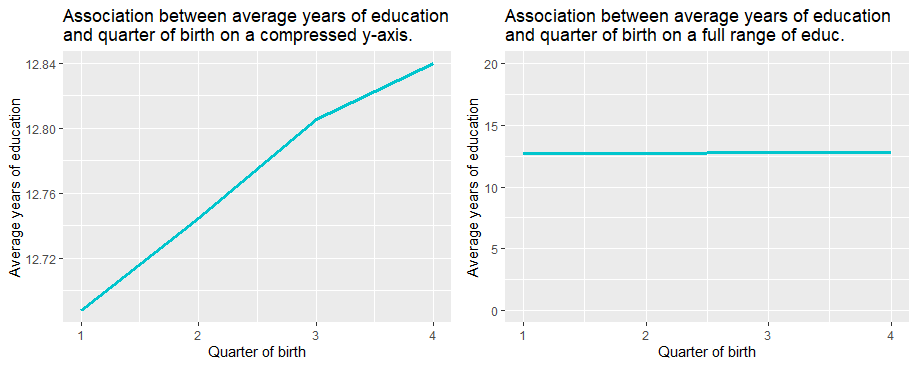
\includegraphics[width=0.7\textwidth]{scatterQobEduc.png}
    \label{fig:qobeduc}
\end{figure}

The same logic should apply to assessing the lack of association between the instrument the explained variable, but the interpretation is flipped around. \hyperref[fig:qobwage]{Figure 5} shows that while on the full range of \textit{lnwage} there is no association with the instrument (on the right), though the compressed y-axis reveals an evident positive association between the two (on the left). 

\begin{figure}[!htbp]
    \caption{Association between the average log-wages and quarter of birth.}
    \centering
    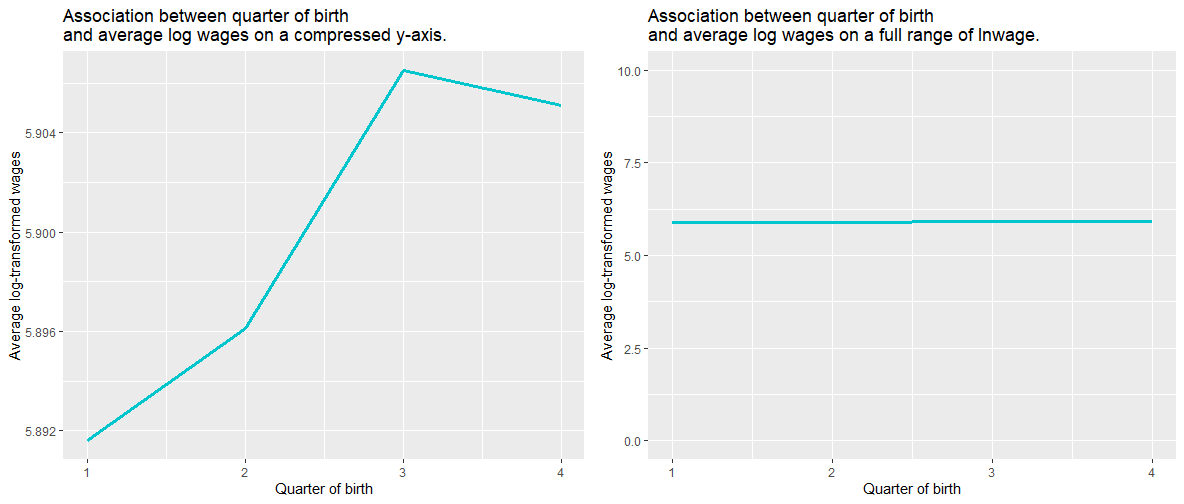
\includegraphics[width=0.67\textwidth]{scatterQobLnwage.png}
    \label{fig:qobwage}
\end{figure}

Lastly, the relevance can be assessed in the light of Pearson's correlation coefficient between \textit{educ} and \textit{qob}. \hyperref[fig:corrplot]{Figure 6} shows the correlation matrix for the variables and instrument in the IV model. The correlation between endogenous variable and the instrument is so low that the colour scale does not depict it (it is in fact equal to 0.01747). This indicates that the instrument is rather not strong. 

\begin{figure}[!htbp]
    \caption{Correlation matrix for variables in rsltSLS.}
    \centering
    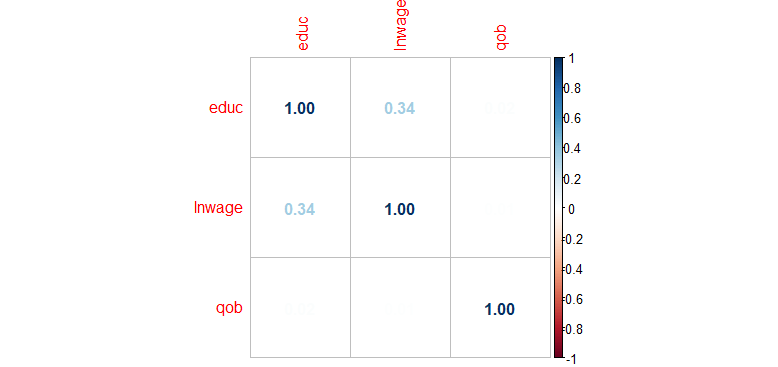
\includegraphics[width=0.55\textwidth]{corrplot.png}
    \label{fig:corrplot}
\end{figure}

In conclusion, the graphical evidence in inconsequential and not congruent with evidence provided by the partial F-test. The relevance criterion cannot be unambiguously determined, although one could lean towards the result of the statistical test. 

\subsection{IV regression analysis of the effect of education on log wages}

The following sections discuss the results of the IV regression specified already in \hyperref[partialftest]{\textit{rsltSLS}} model estimation and the impact of control variables. Further on, the use of robust standard errors is examined in regards to statistical inferences from the model.

\subsubsection{Results}

In \hyperref[tab:ivregresult]{Table 14} results of the IV regression model estimation are presented. Log-transformed wages are regressed on years of education with quarter of birth introduced as an instrumental variables. Interpretation of the estimate is as follows: with an additional year of education, an expected 9.9\% increase in wage is excepted. The result is statistically significant with a p-value $<$ 0.01. Moreover, 9.8\% of variation in log-wages is explained by the predictor (and instrument).   

\begin{table}[!htbp] \centering 
  \caption{Estimation of IV regression model with \textit{qob} as an instrument.} 
  \label{tab:ivregresult} 
\begin{tabular}{@{\extracolsep{5pt}}lD{.}{.}{-3} } 
\\[-1.8ex]\hline 
\hline \\[-1.8ex] 
 & \multicolumn{1}{c}{\textit{Dependent variable:}} \\ 
\cline{2-2} 
\\[-1.8ex] & \multicolumn{1}{c}{lnwage} \\ 
\hline \\[-1.8ex] 
 Constant & 4.633^{***} \\ 
  & (0.250) \\ 
  educ & 0.099^{***} \\ 
  & (0.020) \\ 
 \hline \\[-1.8ex] 
Observations & \multicolumn{1}{c}{329,509} \\ 
R$^{2}$ & \multicolumn{1}{c}{0.098} \\ 
Adjusted R$^{2}$ & \multicolumn{1}{c}{0.098} \\ 
Residual Std. Error & \multicolumn{1}{c}{0.645 (df = 329507)} \\ 
\hline 
\hline \\[-1.8ex] 
\textit{Note:}  & \multicolumn{1}{r}{$^{*}$p$<$0.1; $^{**}$p$<$0.05; $^{***}$p$<$0.01} \\ 
\end{tabular} 
\end{table} 

\subsubsection{Control variables for IV regression}

In this part, additional exogenous regressors (excluding the instrument) are introduced to the model specification. Beside years of education (1), log-wages will now be regressed on marital status and an indicator of living situation in model (2) and age (3) on top of the specification number two. \hyperref[tab:ivregcontrol]{Table 15} shows the results of the estimation and below is the specification of the models under analysis:

\begin{minted}{R}
rsltSLS <- ivreg(lnwage ~ educ | qob, data = dfIVAll)
rsltSLSControl <- ivreg(lnwage ~ educ | qob + married + SMSA, data = dfIVAll)
rsltSLSControl2 <- ivreg(lnwage ~ educ | qob + married + SMSA + age, data = dfIVAll)
\end{minted}

The results are highly interesting. Introducing marital status and living situation to the model specification in (2) just slightly decreases an estimated wage increase of 9.9\% to 9.8\% in response to additional year of education. Over and above to that, being married is associated with an increase of 25.6\% of the wage one earns which is a significant improvement. Living in the urban area corresponds with a decrease of wage by 15.1\% in the model.

Interestingly, when controlling for \textit{age} on top of the marital status and living situation (3), the effect of additional year of education on wage is even stronger - the associated increase in earnings is 15.6\%. However, it is worth noting that the explanatory power of the model denoted by R-squared is negative -3.6\%. This is of high relevance as negative R-squared means that the model built in (3) fits the data worse than a horizontal line which is a null hypothesis for R-squared application. It means that the line representing the linear model hardly follows the trend in the data when adding \textit{age} as control variable.

\begin{table}[!htbp] \centering 
  \caption{Estimation of IV regression model with exogenous regressors as control variables.} 
  \label{tab:ivregcontrol} 
\begin{tabular}{@{\extracolsep{5pt}}lD{.}{.}{-3} D{.}{.}{-3} D{.}{.}{-3} } 
\\[-1.8ex]\hline 
\hline \\[-1.8ex] 
 & \multicolumn{3}{c}{\textit{Dependent variable:}} \\ 
\cline{2-4} 
\\[-1.8ex] & \multicolumn{3}{c}{lnwage} \\ 
\\[-1.8ex] & \multicolumn{1}{c}{(1)} & \multicolumn{1}{c}{(2)} & \multicolumn{1}{c}{(3)}\\ 
\hline \\[-1.8ex] 
 Constant & 4.633^{***} & 4.461^{***} & 3.302^{***} \\ 
  & (0.250) & (0.249) & (0.548) \\ 
  educ & 0.099^{***} & 0.098^{***} & 0.156^{***} \\ 
  & (0.020) & (0.020) & (0.035) \\ 
  married &  & 0.256^{***} & 0.237^{***} \\ 
  &  & (0.006) & (0.011) \\ 
  SMSA &  & -0.151^{***} & -0.085^{**} \\ 
  &  & (0.022) & (0.040) \\ 
  age &  &  & 0.009^{***} \\ 
  &  &  & (0.002) \\ 
 \hline \\[-1.8ex] 
Observations & \multicolumn{1}{c}{329,509} & \multicolumn{1}{c}{329,509} & \multicolumn{1}{c}{329,509} \\ 
R$^{2}$ & \multicolumn{1}{c}{0.098} & \multicolumn{1}{c}{0.124} & \multicolumn{1}{c}{-0.036} \\ 
Adjusted R$^{2}$ & \multicolumn{1}{c}{0.098} & \multicolumn{1}{c}{0.124} & \multicolumn{1}{c}{-0.036} \\ 
Residual Std. Error & \multicolumn{1}{c}{0.645 (df = 329507)} & \multicolumn{1}{c}{0.635 (df = 329505)} & \multicolumn{1}{c}{0.691 (df = 329504)} \\ 
\hline 
\hline \\[-1.8ex] 
\textit{Note:}  & \multicolumn{3}{r}{$^{*}$p$<$0.1; $^{**}$p$<$0.05; $^{***}$p$<$0.01} \\ 
\end{tabular} 
\end{table} 

\subsubsection{Robust standard errors for IV regression}

In this section robust standard errors are applied to examine whether the statistical significance of estimates is affected by the more conservative approach to standard errors' computation.

\begin{table}[!htbp] \centering 
  \caption{Estimation of IV regression model with (1) basic SE, (2) White's SE and (3) clustered SE on \textit{age}.} 
  \label{tab:ivregrobust} 
\begin{tabular}{@{\extracolsep{5pt}}lD{.}{.}{-3} D{.}{.}{-3} D{.}{.}{-3} } 
\\[-1.8ex]\hline 
\hline \\[-1.8ex] 
 & \multicolumn{3}{c}{\textit{Dependent variable:}} \\ 
\cline{2-4} 
\\[-1.8ex] & \multicolumn{3}{c}{lnwage} \\ 
\\[-1.8ex] & \multicolumn{1}{c}{(1)} & \multicolumn{1}{c}{(2)} & \multicolumn{1}{c}{(3)}\\ 
\hline \\[-1.8ex] 
 Constant & 4.461^{***} & 4.461^{***} & 4.461^{***} \\ 
  & (0.248600) & (0.249039) & (0.249042) \\ 
  educ & 0.098^{***} & 0.098^{***} & 0.098^{***} \\ 
  & (0.019529) & (0.019559) & (0.019559) \\ 
  married & 0.256^{***} & 0.256^{***} & 0.256^{***} \\ 
  & (0.006488) & (0.006669) & (0.006670) \\ 
  SMSA & -0.151^{***} & -0.151^{***} & -0.151^{***} \\ 
  & (0.021990) & (0.022047) & (0.022047) \\ 
 \hline \\[-1.8ex] 
Observations & \multicolumn{1}{c}{329,509} & \multicolumn{1}{c}{329,509} & \multicolumn{1}{c}{329,509} \\ 
R$^{2}$ & \multicolumn{1}{c}{0.124} & \multicolumn{1}{c}{0.124} & \multicolumn{1}{c}{0.124} \\ 
Adjusted R$^{2}$ & \multicolumn{1}{c}{0.124} & \multicolumn{1}{c}{0.124} & \multicolumn{1}{c}{0.124} \\ 
Residual Std. Error (df = 329505) & \multicolumn{1}{c}{0.635} & \multicolumn{1}{c}{0.635} & \multicolumn{1}{c}{0.635} \\ 
\hline 
\hline \\[-1.8ex] 
\textit{Note:}  & \multicolumn{3}{r}{$^{*}$p$<$0.1; $^{**}$p$<$0.05; $^{***}$p$<$0.01} \\ 
\end{tabular} 
\end{table}

Results are available in \hyperref[tab:ivregrobust]{Table 16}. As can be expected given the explanation of robust SEs computation in \hyperref[controlrobustDID]{this section}, the more conservative the method the higher the standard errors. It is worth noting that the differences were so small that they could have been omitted due to the rounding. \hyperref[tab:ivregrobust]{Table 16} is evidently displaying more digits for standard errors than usually. Increased standard errors do not affect estimates (by definition) and their statistical significance, so it can be concluded that the statistical inference is not affected by introduction of robust standard errors.


\subsection{OLS estimation and IV}

In this section appropriate formal tests will be applied to decide between the OLS- and IV-estimated models and to examine if over-identification is the issue in the IV model with control variables.

\subsubsection{Testing the validity of using OLS- and IV-estimated models}

For the purpose of deciding between OLS an IV models a specification of the OLS estimation is necessary (presented with an IV model already introduced):

\begin{minted}{R}
rsltSLS <- ivreg(lnwage ~ educ | qob, data = dfIVAll)
rsltOLS <- lm(lnwage ~ educ, data = dfIVAll)
\end{minted}

\hyperref[tab:ivregols]{Table 17} looks at the results of the OLS- and IV-estimated models. The effect of education on the explained variable is lower in OLS model than in IV model, but still indicated a positive relationship and increase of wages by 7.1\% with additional unit of education. The explanatory power of the models in terms or R-squared is lower for the IV-estimated model, though the significance of estimates in both models in terms of p-value is strong (p-value $<$ 0.01).

\begin{table}[!htbp] \centering 
  \caption{Estimation of OLS- and IV-estimated regression model.} 
  \label{tab:ivregols} 
\begin{tabular}{@{\extracolsep{5pt}}lD{.}{.}{-3} D{.}{.}{-3} } 
\\[-1.8ex]\hline 
\hline \\[-1.8ex] 
 & \multicolumn{2}{c}{\textit{Dependent variable:}} \\ 
\cline{2-3} 
\\[-1.8ex] & \multicolumn{2}{c}{lnwage} \\ 
\\[-1.8ex] & \multicolumn{1}{c}{\textit{OLS}} & \multicolumn{1}{c}{\textit{instrumental}} \\ 
 & \multicolumn{1}{c}{\textit{}} & \multicolumn{1}{c}{\textit{variable}} \\ 
\\[-1.8ex] & \multicolumn{1}{c}{(1)} & \multicolumn{1}{c}{(2)}\\ 
\hline \\[-1.8ex] 
 Constant & 4.995^{***} & 4.633^{***} \\ 
  & (0.004) & (0.250) \\ 
  educ & 0.071^{***} & 0.099^{***} \\ 
  & (0.0003) & (0.020) \\ 
 \hline \\[-1.8ex] 
Observations & \multicolumn{1}{c}{329,509} & \multicolumn{1}{c}{329,509} \\ 
R$^{2}$ & \multicolumn{1}{c}{0.117} & \multicolumn{1}{c}{0.098} \\ 
Adjusted R$^{2}$ & \multicolumn{1}{c}{0.117} & \multicolumn{1}{c}{0.098} \\ 
Residual Std. Error (df = 329507) & \multicolumn{1}{c}{0.638} & \multicolumn{1}{c}{0.645} \\ 
F Statistic & \multicolumn{1}{c}{43,782.560$^{***}$ (df = 1; 329507)} &  \\ 
\hline 
\hline \\[-1.8ex] 
\textit{Note:}  & \multicolumn{2}{r}{$^{*}$p$<$0.1; $^{**}$p$<$0.05; $^{***}$p$<$0.01} \\ 
\end{tabular} 
\end{table} 

The suitability of either of the models will be examined with a use of Hausman's test. It assesses the assumed exogeneity of the independent variable in order to decide if instrumental variable estimation is required. Results in \hyperref[tab:hausman]{Table 18} uncover the p-value of the Hausman's test to be equal to 0.143. The null hypothesis cannot be rejected which means that assumed exogeneity cannot be maintained and and one should use OLS to estimate the desired model.

\begin{table}[!htbp] \centering 
  \caption{Diagnostics for the IV-estimated model - Hausman's test.} 
  \label{tab:hausman} 
\begin{tabular}{rrrrr}
  \hline
 & df1 & df2 & statistic & p-value \\ 
  \hline
  Wu-Hausman & 1.00 & 329506.00 & 2.144 & 0.143 \\ 
   \hline
\end{tabular}
\end{table}

\subsubsection{Over-identification}

In this section issues caused by over-identification are put to test with the use of Sargan's test. It evaluates the assumed cleanness of instruments - extra equations that arise from having more instruments than endogenous variables are considered. IV regression model with quarter of birth, marital status and indicator of living situation as instruments is tested. Results in \hyperref[tab:sargan]{Table 19} uncover p-value to be very low (p-value $<$ 0.001) which means enough evidence to reject the null hypothesis. This result informs the recipient that some of the instruments must be removed because the cleanness of instruments is violated with an over-identification of the model.

\begin{table}[!htbp] \centering 
  \caption{Diagnostics for the IV-estimated model - Sargan's test.} 
  \label{tab:sargan} 
\begin{tabular}{rrrrr}
  \hline
 & df1 & df2 & statistic & p-value \\ 
  \hline 
  Sargan & 2.00 &  & 2262.01 & $<$2e-16 \\ 
   \hline
\end{tabular}
\end{table}


\subsection{Shortcomings of \emph{qob} as an identified instrument}

This section elaborates on possible causes of concern that could in principle render \textit{qob} invalid as an identified instrumental variable.

The relationship of age gaps between the classmates/students and their results in school and satisfaction of said results is very important to consider when choosing quarter of birth as an instrument for effects of additional education on any aspects of life. This is especially relevant for schooling in early stages of life where age gaps between pupils in the same class/cohort are only of a few months. Older children develop faster which gives them a natural advantage over children born later in a given year. Such advantages then translate to better achievements in education and consequently higher joy and satisfaction a child will have when attending school. This can be a motive for an older child to pursue higher education and generally be more ambitious, and for younger child to abandon school earlier and not rip the benefits of additional years of education.

A second argument takes into account a consideration of a particular subject missing his or her window to enter a school cohort corresponding with subject's age. If there are people (mostly children as it applies in the early stage education) that for whatever reason systematically miss the admission year of their peers, then there are older subjects systematically entering a population of younger people. Hence people that are older will be developing and entering new stages in life (and therefore having other achievements faster or more seamlessly) earlier than other, though they will still be considered in the same quarter of births.

\newpage

\appendix

\section{Appendix - code}
\begin{tiny}
\begin{minted}{R}


############################################################################
############################################################################
###                                                                      ###
###                ALEKSANDER ODZIEMKOWSKI, BAM01 AS&P                   ###
###                INDIVIDUAL ASSIGNMENT 2, 28.09.2022                   ###
###                                                                      ###
############################################################################
############################################################################


##################################################################
##              Setting up the IDE and environment              ##
##################################################################

# ----------------------------------
# Clear the console and environment
# ----------------------------------
remove(list=ls())
cat("\f")

# ---------
# Packages
# ---------
library(stargazer)
library(corrplot)
library(lm.beta)
library(knitr)
library(gridExtra)
library(tidyverse)
library(plyr)
library(reshape2)
library(ggplot2)
library(olsrr)
library(lm.beta)
library(sandwich)
library(car)
library(bannerCommenter)
library(AER)
library(xtable)
library(ivreg)

# ----------------------------------------------------
# Set working directory and define folder's structure
# ----------------------------------------------------
setwd("C:/STUDIA - materiały/RSM-MASTERS/COURSES/BLOCK 1/Advanced Statistics and Programming/Assignment 2")

dir <- "C:/STUDIA - materiały/RSM-MASTERS/COURSES/BLOCK 1/Advanced Statistics and Programming/Assignment 2/"

dirData <- paste0(dir, "Data/")
dirProg <- paste0(dir, "Programs/")
dirRslt <- paste0(dir, "Results/")


##################################################################
##        Difference-in-Difference analysis: female labor       ##
##                    force participation                       ##
##################################################################


#################################################################
##              Import and inspect the DiD data                ##
#################################################################

# -----------------------------------
# Import CSV data - DiD_dataset.csv
# -----------------------------------
options(digits=7)

dfDiDAll <- read.csv(file = paste0(dirData, "DiD_dataset.csv"), header = TRUE, stringsAsFactors = FALSE)


# Checking n/a per variable as linear regression model will not handle missing values;
dfMissingValues <- as.data.frame(colSums(is.na(dfDiDAll)))
colnames(dfMissingValues) <- c("# Missing Values")
# Conclusion - no missing values, dataset is complete

str(dfDiDAll)
# Conclusion - all variables seem to have a correct data type


# -----------------------------------
# Data manipulation and cleaning
# -----------------------------------

# Introduce the period indicator
dfDiDAll$dPeriod <- ifelse(dfDiDAll$year < 1993, 0, 1)

# Introduce a dummy variable for a presence of children
dfDiDAll$dChildren <- ifelse(dfDiDAll$children == 0, 0, 1)

# Take a look at possible duplicates 
dfDiDDuplicates <- as.data.frame(dfDiDAll[duplicated(dfDiDAll),])
# Conclusion- there are 20 duplicates but their nature cannot be conveniently assessed



#################################################################
##              Equations and their adjustment                 ##
#################################################################


#' Y <- the effect; dfDiDAll$work
#' T0 <- pre-effect-period; dfDiDAll$year in 1991, 1992
#' T1 <- post-effect-period; dfDiDAll$year in 1993 and beyond
#' D0 <- no children; dfDiDAll$dChildren = 0
#' D1 <- had children; dfDiDAll$dChildren = 1
#' 
#' State id or state's unemployment rate can be added as a control variable to account for local labor market effects



##################################################################################
##              Plots as visual evidence of the DiD effect of the EITC          ##
##       by means of annual earnings, annual family and working/non-working     ##
##################################################################################

# 1) Annual earnings
lineEarnEffect <- ggplot(dfDiDAll, aes(x = year, y = earn, group = dChildren, color = dChildren))

lineEarnEffect + 
  stat_summary(geom = "line", fun = mean, lwd=1.2) +
  labs(x = "Year", y = "Annual earnings") +
  geom_vline(xintercept=as.numeric(1993), linetype = 4) +
  scale_colour_gradient(limits = c(0, 1), 
                        breaks = c(0, 1),
                        labels = c(0, 1)) +
  theme(legend.position="right")

# ggsave(paste0(dirRslt, "lineEarnEffect.png"), width = 11, height = 6)

# 2) Family income
lineFincEffect <- ggplot(dfDiDAll, aes(x = year, y = finc, group = dChildren, color = dChildren))

lineFincEffect + 
  stat_summary(geom = "line", fun = mean, lwd=1.2) +
  labs(x = "Year", y = "Family earnings") +
  geom_vline(xintercept=as.numeric(1993), linetype = 4) +
  scale_colour_gradient(limits = c(0, 1), 
                        breaks = c(0, 1),
                        labels = c(0, 1)) +
  theme(legend.position="right")

# ggsave(paste0(dirRslt, "lineFincEffect.png"), width = 11, height = 6)

# 3) Work indicator
lineWorkEffect <- ggplot(dfDiDAll, aes(x = year, y = work, group = dChildren, color = dChildren))

lineWorkEffect + 
  stat_summary(geom = "line", fun = mean, lwd=1.2) +
  labs(x = "Year", y = "Indicator of work status (proportion)") +
  geom_vline(xintercept=as.numeric(1993), linetype = 4) +
  scale_colour_gradient(limits = c(0, 1), 
                        breaks = c(0, 1),
                        labels = c(0, 1)) +
  theme(legend.position="right")

# ggsave(paste0(dirRslt, "lineWorkEffect.png"), width = 11, height = 6)

##################################################################################
##              Stargazer to provide a table with summary statistics            ##
##                and concise description of the data in the table              ##
##################################################################################

order = which(names(dfDiDAll)%in%c("urate", "finc", "earn", "unearn", "age", "ed", "work", "children", "dChildren", "nonwhite", "dPeriod"))

stargazer(dfDiDAll, 
          summary.stat = c("mean", "sd", "min", "p25", "median", "p75", "max"), 
          omit = c("state", "year"), 
          digits = 2,
          order = order,
          type = 'text'
          )


##################################################################################
##              Provide matrices of three difference-in-differences             ##
##                effects of EITC introduction per each variable                ##
##################################################################################

# -----------------------------------
# Indicator of work status
# -----------------------------------

# Prepare the means
avgEmpl <- ddply(dfDiDAll, .(dPeriod, dChildren), summarise,
                 avgEmploy = mean(work))

# Make table for the outcomes
tmp <- dcast(avgEmpl, dPeriod ~ dChildren, value.var = 'avgEmploy')
tmp <- rbind(tmp, tmp[2,]-tmp[1,])

# Rename the rows and columns
rownames(tmp) <- c("Pre-effect", "Post-effect", "Difference")
colnames(tmp) <- c("dPeriod", "No children", "Had children")
tmp[3, "dPeriod"] <- NA

# Table with the results
stargazer(tmp, summary = FALSE, align = TRUE, type = 'text')


# -----------------------------------
# Annual earnings
# -----------------------------------

# Prepare the means
avgEarn <- ddply(dfDiDAll, .(dPeriod, dChildren), summarise,
                 avgEarn = mean(earn))

# Make table for the outcomes
tmpEarn <- dcast(avgEarn, dPeriod ~ dChildren, value.var = 'avgEarn')
tmpEarn <- rbind(tmpEarn, tmpEarn[2,]-tmpEarn[1,])

# Rename the rows
rownames(tmpEarn) <- c("Pre-effect", "Post-effect", "Difference")
colnames(tmpEarn) <- c("dPeriod", "No children", "Had children")
tmpEarn[3, "dPeriod"] <- NA


# Table with the results
stargazer(tmpEarn, summary = FALSE, align = TRUE, type = 'text')


# -----------------------------------
# Family annual income
# -----------------------------------

# Prepare the means
avgFinc <- ddply(dfDiDAll, .(dPeriod, dChildren), summarise,
                  avgFinc = mean(finc))

# Make table for the outcomes
tmpFinc <- dcast(avgFinc, dPeriod ~ dChildren, value.var = 'avgFinc')
tmpFinc <- rbind(tmpFinc, tmpFinc[2,]-tmpFinc[1,])

# Rename the rows
rownames(tmpFinc) <- c("Pre-effect", "Post-effect", "Difference")
colnames(tmpFinc) <- c("dPeriod", "No children", "Had children")
tmpFinc[3, "dPeriod"] <- NA


# Table with the results
stargazer(tmpFinc, summary = FALSE, align = TRUE, type = 'text')

##################################################################################
##              Regression models for the three dependent variables.            ##
##  What is the effect of the policy introduction on the dependent variables?   ##
##            How does the effect change when adding control variables?         ##
##                      Are robust standard errors necessary?                   ##
##################################################################################

# ------------------------------------------------------------------------
# Running the actual difference-in-difference model and getting estimates
# ------------------------------------------------------------------------

# Define models
mdlWork <- work ~ dChildren + dPeriod +dChildren:dPeriod
mdlEarn <- earn ~ dChildren + dPeriod +dChildren:dPeriod
mdlFinc <- finc ~ dChildren + dPeriod +dChildren:dPeriod

# Estimate models
rstlOLSWork <- lm(mdlWork, data = dfDiDAll)
rstlOLSEarn <- lm(mdlEarn, data = dfDiDAll)
rstlOLSFinc <- lm(mdlFinc, data = dfDiDAll)


# The summary table
stargazer(rstlOLSWork, rstlOLSEarn, rstlOLSFinc,
          intercept.bottom = FALSE, align = TRUE, no.space = TRUE,
          type = 'text')


# -------------------------
# Adding control variables
# -------------------------

mdlWorkControl <- work ~ dChildren + dPeriod +dChildren:dPeriod + urate + nonwhite
mdlEarnControl <- earn ~ dChildren + dPeriod +dChildren:dPeriod + urate + nonwhite
mdlFincControl <- finc ~ dChildren + dPeriod +dChildren:dPeriod + urate + nonwhite

rstlOLSWorkControl <- lm(mdlWorkControl, data = dfDiDAll)
rstlOLSEarnControl <- lm(mdlEarnControl, data = dfDiDAll)
rstlOLSFincControl <- lm(mdlFincControl, data = dfDiDAll)

stargazer(rstlOLSWorkControl, rstlOLSEarnControl, rstlOLSFincControl,
          intercept.bottom = FALSE, align = TRUE, no.space = TRUE,
          type = 'text')


# --------------
# Robust errors
# --------------

# Remedy for heteroscedasticity - robust standard errors (they are more conservative)
# Check if introducing robust errors increase the value of standard errors

# Work indicator
seBasicWork <- sqrt(diag(vcov(rstlOLSWork)))
seWhiteWork <- sqrt(diag(vcovHC(rstlOLSWork, type = 'HC0')))
seClustWork <- sqrt(diag(vcovHC(rstlOLSWork, cluster = 'state')))

stargazer(rstlOLSWork, rstlOLSWork, rstlOLSWork, se = list(seBasicWork, seWhiteWork, seClustWork),
          intercept.bottom = FALSE, align = TRUE, no.space = TRUE, 
          type = 'text')

# Earnings
seBasicEarn <- sqrt(diag(vcov(rstlOLSEarn)))
seWhiteEarn <- sqrt(diag(vcovHC(rstlOLSEarn, type = 'HC0')))
seClustEarn <- sqrt(diag(vcovHC(rstlOLSEarn, cluster = 'state')))

stargazer(rstlOLSEarn, rstlOLSEarn, rstlOLSEarn, se = list(seBasicEarn, seWhiteEarn, seClustEarn),
          intercept.bottom = FALSE, align = TRUE, no.space = TRUE, 
          type = 'text')


# Family income
seBasicFinc <- sqrt(diag(vcov(rstlOLSFinc)))
seWhiteFinc <- sqrt(diag(vcovHC(rstlOLSFinc, type = 'HC0')))
seClustFinc <- sqrt(diag(vcovHC(rstlOLSFinc, cluster = 'state')))

stargazer(rstlOLSFinc, rstlOLSFinc, rstlOLSFinc, se = list(seBasicFinc, seWhiteFinc, seClustFinc),
          intercept.bottom = FALSE, align = TRUE, no.space = TRUE, 
          type = 'text')


##################################################################################
##     Do high-education mothers react differently to the EITC policy measure   ##
##                than low education mothers? 9 years as a threshold            ##
##                          in terms of length of education                     ##
##################################################################################

# Estimate models:

# Single mothers with high education and with children. Compare
# them with single mothers with low education and with children.

#Introducing a dummy variable for differentiating between high ed and low ed
dfDiDAll$dHighEd <- ifelse(dfDiDAll$ed < 9, 0, 1)

mdlWorkHaveChild <- work ~ dHighEd + dPeriod + dHighEd:dPeriod
mdlEarnHaveChild <- earn ~ dHighEd + dPeriod + dHighEd:dPeriod
mdlFincHaveChild <- finc ~ dHighEd + dPeriod + dHighEd:dPeriod

rstlOLSWorkHaveChild <- lm(mdlWorkHaveChild, data = dfDiDAll, subset = (dfDiDAll$children == 1))
rstlOLSEarnHaveChild <- lm(mdlEarnHaveChild, data = dfDiDAll, subset = (dfDiDAll$children == 1))
rstlOLSFincHaveChild <- lm(mdlFincHaveChild, data = dfDiDAll, subset = (dfDiDAll$children == 1))

a1 <- rstlOLSWork
a2 <- rstlOLSWorkHaveChild
b1 <- rstlOLSEarn
b2 <- rstlOLSEarnHaveChild
c1 <- rstlOLSFinc
c2 <-rstlOLSFincHaveChild

stargazer(a2, b2, c2,
          intercept.bottom = FALSE, align = TRUE, no.space = TRUE,
          type = 'text')

stargazer(a1, a2,
          intercept.bottom = FALSE, align = TRUE, no.space = TRUE,
          type = 'text')

stargazer(b1, b2,
          intercept.bottom = FALSE, align = TRUE, no.space = TRUE,
          type = 'text')

stargazer(c1, c2,
          intercept.bottom = FALSE, align = TRUE, no.space = TRUE,
          type = 'text')


# Single women with low education, without children. Compare them
# with single women with low education, with children.

mdlWorkLowEd <- work ~ dChildren + dPeriod +dChildren:dPeriod
mdlEarnLowEd <- earn ~ dChildren + dPeriod +dChildren:dPeriod
mdlFincLowEd <- finc ~ dChildren + dPeriod +dChildren:dPeriod

rstlOLSWorkLowEd <- lm(mdlWorkLowEd, data = dfDiDAll, subset = (dfDiDAll$dHighEd == 0))
rstlOLSEarnLowEd <- lm(mdlEarnLowEd, data = dfDiDAll, subset = (dfDiDAll$dHighEd == 0))
rstlOLSFincLowEd <- lm(mdlFincLowEd, data = dfDiDAll, subset = (dfDiDAll$dHighEd == 0))

stargazer(rstlOLSWorkLowEd, rstlOLSEarnLowEd, rstlOLSFincLowEd,
          intercept.bottom = FALSE, align = TRUE, no.space = TRUE,
          type = 'text')



##################################################################
##                Instrumental Variable analysis:               ##
##            effect of compulsory schooling on wages           ##
##################################################################


#################################################################
##              Import and inspect the IV data                 ##
#################################################################

# -----------------------------------
# Import CSV data - IV_dataset.csv
# -----------------------------------

dfIVAll <- read.csv(file = paste0(dirData, "IV_dataset.csv"), header = TRUE, stringsAsFactors = FALSE)

# Select only the variables that are mentioned in the task
dfIVAll <- 
  dfIVAll %>%
  select(age, educ, lnwage, married, qob, SMSA, yob)

# Checking n/a per variable as linear regression model will not handle missing values;
dfMissingValuesIV <- as.data.frame(colSums(is.na(dfIVAll)))
colnames(dfMissingValuesIV) <- c("# Missing Values")
# Conclusion - no missing values, dataset is complete

str(dfIVAll)
# Conclusion - structure is correct


#################################################################
##        Task 2: Summary statistics and concise descrp        ##
#################################################################
order1 = which(names(dfIVAll)%in%c("lnwage", "age", "educ", "married", "qob", "yob", "SMSA"))

stargazer(dfIVAll, 
          summary.stat = c("mean", "sd", "min", "p25", "median", "p75", "max"), 
          digits = 2,
          order = order1,
          type = 'text')

#################################################################
##                            Task 3:                          ##
##    Explore if variable qob meets the relevance criterion    ##
##        as a good instrument for years of education          ##
#################################################################

# Relevance: need to have sufficiently strong correlation 
# between the instrument and the instrumentalized variables

# -------------
# Regressions 
# -------------

# partial F-test - run the iv regression and perform diagnostics 
# to assess the strength of the instrument
rsltSLS <- ivreg(lnwage ~ educ | qob,
                 data = dfIVAll)

stargazer(rsltSLS, 
          intercept.bottom = FALSE, align = TRUE, no.space = TRUE,
          type = 'text')

summ.ivreg <- summary(rsltSLS, diagnostics = TRUE)

xtable(summ.ivreg$diagnostics)

# -----------------------
# Plot of QOB relevance
# -----------------------

scatterQobEduc <- ggplot(data = dfIVAll, aes(x = qob, y = educ))

ad <- scatterQobEduc +
  stat_summary(geom = "line", fun = mean, lwd=1.2, color = "turquoise3") +
  labs(x = "Quarter of birth", y = "Average years of education") +
  theme(legend.position="bottom") +
  ggtitle(label = "Association between average years of education \nand quarter of birth on a compressed y-axis.")

bo <- scatterQobEduc +
  stat_summary(geom = "line", fun = mean, lwd=1.2, color = "turquoise3") +
  labs(x = "Quarter of birth", y = "Average years of education") +
  theme(legend.position="bottom") +
  ylim(0,20) +
  ggtitle(label = "Association between average years of education \nand quarter of birth on a full range of educ.")

# Combine graphs with gridExtra
grid.arrange(ad, bo, ncol=2, nrow =1)

# ggsave(paste0(dirRslt, "scatterQobEduc.png"), width = 11, height = 8)


scatterQobLnwage <- ggplot(data = dfIVAll, aes(x = qob, y = lnwage))

ca <- scatterQobLnwage +
  stat_summary(geom = "line", fun = mean, lwd=1.2, color = "turquoise3") +
  labs(x = "Quarter of birth", y = "Average log-transformed wages") +
  theme(legend.position="bottom") +
  ggtitle(label = "Association between quarter of birth \nand average log wages on a compressed y-axis.")

hu <- scatterQobLnwage +
  stat_summary(geom = "line", fun = mean, lwd=1.2, color = "turquoise3") +
  labs(x = "Quarter of birth", y = "Average log-transformed wages") +
  theme(legend.position="bottom") +
  ylim(0,10) +
  ggtitle(label = "Association between quarter of birth \nand average log wages on a full range of lnwage.")

# Combine graphs with gridExtra
grid.arrange(ca, hu, ncol=2, nrow =1)

# ggsave(paste0(dirRslt, "scatterQobLnwage.png"), width = 11, height = 8)

# Correlation matrix
cor(dfIVAll$educ, dfIVAll$qob)

subset_cor <- 
  dfIVAll %>%
  select(educ, lnwage, qob)

corrplot(cor(subset_cor), method = "number")
# ggsave(paste0(dirRslt, "corrplot.png"), width = 11, height = 8)

# Correlation coefficient - too low to display in the matrix
cor(dfIVAll$educ, dfIVAll$qob)


#######################################################################
##                               Task 4:                             ## 
##  IV regression analysis of the effect of education on log wages,  ##
##             using quarter of birth as the instrument.             ##
##  What is the effect of an additional year of education on wages?  ##
#######################################################################

rsltSLS <- ivreg(lnwage ~ educ | qob,
                      data = dfIVAll)

stargazer(rsltSLS, 
          intercept.bottom = FALSE, align = TRUE, no.space = TRUE,
          type = 'text')

summary(rsltSLS, diagnostics = TRUE)

####################################################################################################
##                   How does the effect change when adding control variables?                    ##
##  Examine if the use of robust standard errors critically affects your statistical inferences.  ##
####################################################################################################

# Adding control variables / exogenous regressors 
rsltSLSControl <- ivreg(lnwage ~ educ | qob + married + SMSA,
                         data = dfIVAll)

rsltSLSControl2 <- ivreg(lnwage ~ educ | qob + married + SMSA + age,
                        data = dfIVAll)

stargazer(rsltSLS, rsltSLSControl, rsltSLSControl2,
          intercept.bottom = FALSE, align = TRUE, no.space = TRUE,
          type = 'text')

# Robust standard errors
seBasicSLS <- sqrt(diag(vcov(rsltSLSControl)))
seWhiteSLS <- sqrt(diag(vcovHC(rsltSLSControl, type = 'HC0')))
seClustSLS <- sqrt(diag(vcovHC(rsltSLSControl, cluster = 'age')))

stargazer(rsltSLSControl, rsltSLSControl, rsltSLSControl, se = list(seBasicSLS, seWhiteSLS, seClustSLS),
          intercept.bottom = FALSE, align = TRUE, no.space = TRUE, 
          type = 'text')

# Notice a slight difference that can be omitted due to rounding in stargazer output
print(seBasicSLS)
print(seWhiteSLS)
print(seClustSLS)


###########################################################################################
##  Following the previous analysis, conduct the same regressions with OLS as with IV.   ##
##      Apply a formal test to decide between the two OLS and IV-estimated models.       ##
##          Examine if over-identification can be an issue in the IV analysis.           ##
###########################################################################################

rsltOLS <- lm(lnwage ~ educ,
              data = dfIVAll)

stargazer(rsltOLS, rsltSLS, 
          intercept.bottom = FALSE, align = TRUE, no.space = TRUE,
          type = 'text')

# Formal test - OLS or IV? 
summ.hausman <- summary(rsltSLS, diagnostics = TRUE)

xtable(summ.hausman$diagnostics)

# Formal test - is over-identification an issue? 

summ.sagan <- summary(rsltSLSControl, diagnostics = TRUE)

xtable(summ.sagan$diagnostics)


\end{minted}
\end{tiny}




\end{document}
